\documentclass[amsmath,amssymb,a4]{revtex4-2}
% updated from revtex4 tot revtex4-2 because revtex4 would cause compiler malfunctioning in the most recent Miktex package. It is superseded by revtex4-2 (https://journals.aps.org/revtex/revtex-faq) so that was used as of 12-2-2020.
\usepackage{graphicx}
\usepackage{longtable}
\usepackage{placeins}
\begin{document}

\title[DIV1D manual]{DIV1D manual: a 1D code for divertor plasma simulation \\ extended with reservoirs}

\author{E. Westerhof}
\author{G.L. Derks}
  \author{S.P. Kobussen}
  

    
\address{DIFFER -- Dutch Institute for Fundamental Energy Research, PO Box 6336, 5600HH Eindhoven, The Netherlands, www.differ.nl}

\email[E-mail: ]{e.westerhof@differ.nl}
\vspace{10pt}
\date\today


% \begin{abstract}
% Abstract goes here.
% \end{abstract}


\maketitle

Copyright (C)  2023  DIFFER.
    Permission is granted to copy, distribute and/or modify this document
    under the terms of the GNU Free Documentation License, Version 1.3
    or any later version published by the Free Software Foundation;
    with no Invariant Sections, no Front-Cover Texts, and no Back-Cover Texts.
    A copy of the license is included in the section entitled "GNU
    Free Documentation License".
    
\section{Introduction}

This manual describes the {\tt DIV1D} code for the quick simulation of the 1D plasma and neutral behaviour along a flux tube in a tokamak divertor from the target/stagnation/X-point up to the target \cite{derks2022}. The code is inspired by similar works described in the papers by Nakazawa et al.~\cite{nakazawa2000} and Dudson et al.~\cite{dudson2019, SD1D}. In fact, the numerical implementation borrows heavily from the methods used in the SD1D code. The code is maintained on a Git repository at DIFFER. This document describes the basic model equations in Section~\ref{basic_equations} including the boundary conditions and the sources and sinks. Section~\ref{rates} contains a full description of the different choices that are implemented to calculate the various atomic processes like charge exchange, ionization, recombination, and impurity radiation. Some notes on the discretization and the numerical implementation are given in Section~\ref{numerics}.


\section{Equations}\label{basic_equations}
The DIV1D is written to solve a fixed set of equations in a modular way. The main equations are postulated for the scrape-off layer. Additionally, DIV1D can solve for equations of external reservoirs for the neutral surroundings and core. Every single equation in this section contains a switch and can be turned on- or off. For self-consistent results it is important that the terms that are not evolved are initialized small such that all interactions with other equations drop out. It is advised for the scrape-off layer to evolve all equations if possible, for the reservoirs the interactions are almost trivial. The following subsections will go through the equations and are followed by components in these equations.

\subsection{Scrape-off layer}
The equations solved are: the particle balance equation, the plasma momentum balance, the plasma energy balance, equations for the evolution of the atomic particle density and velocity as well as an equation for the molecule particle balance.

\noindent The particle balance is given by
\begin{equation}\label{particle_balance}
    {\partial n \over \partial t} = - B{\partial \over \partial x} \left({\Gamma_n \over B}\right) + S_n,
\end{equation}
where $n$ is the plasma (electron) density, $\Gamma_n = n v_\parallel$ with $v_\parallel$ the parallel velocity is the convective particle flux (a possible effect of diffusion is ignored), and $S_n$ represent the sum of all particle sources and sinks. $B$ represents the magnitude of the total magnetic field. Here and in the equations below, the inclusion of $B$ accounts for the effect of flux expansion due to a varying total magnetic field~\cite{dudson2019,havlickova2013}.

\noindent The momentum balance is given by
\begin{equation}\label{momentum_balance}
    {\partial n m v_\parallel \over \partial t} = - B{\partial \over \partial x} \left({n m v_\parallel^2 \over B}\right) - {\partial \over \partial x} p + S_{\rm mom},
\end{equation}
where $m$ is the mass of the dominant ion species (default Deuterium $m = 3.3436 \times 10^{-27}$~kg) , $p = 2 n e T$ is the total plasma pressure (we will use T in units eV such that the Boltzmann constant can be equated with the elementary charge $e$ to obtain the pressure in Pascal), and $S_{\rm mom}$ represent the sum of all momentum sources and sinks.

\noindent Ion and electron temperatures are considered equal such that only one energy balance needs to be solved. The internal energy ($3 n k T$) balance of the plasma is then given by
\begin{equation}\label{energy_balance}
    {\partial 3 n e T \over \partial t} = - B{\partial \over \partial x} \left({q_\parallel \over B}\right) + v_\parallel {\partial \over \partial x} p + Q,
\end{equation}
where the heat flux $q_\parallel$ is given by the equation
\begin{equation}\label{heat_flux}
    q_\parallel = 5 n e T v_\parallel - \kappa_\parallel {\partial \over \partial x} T,
\end{equation}
where the first term on the right hand side represents the total enthalpy flux and the second term represents the parallel heat conduction with (for T in eV) the parallel conductivity being given by $\kappa_\parallel = 2 \times 10^3 T^{5/2}$ J/eVms (see Chapter 4.10.1 of \cite{stangeby}). $Q$ represent the sum of all internal energy sources and sinks.

\noindent The neutral particle balance is given by
\begin{equation}\label{eq:neutral density}
    {\partial n_a \over \partial t} = {\partial \over \partial x} \left( D_a {\partial \over \partial x} n_a \right)- {\partial \over \partial x}(n_a v_a) + S_{\rm a},%\quad \mathrm{[m^{-3}s^{-1}]},
\end{equation}
where $n_a$ is the atomic particle density, $v_a$ the atom bulk velocity, and $D_a$ is the atom particle diffusion coefficient which is given by \cite{nakazawa2000}
\begin{equation}\label{neutral_diffusion_coefficient}
    D_a = { e\sqrt{TT_a} \over m (\nu_{\rm cx}+\nu_{\rm el}) \sin^2\theta }
\end{equation}
where $\theta$ is the angle at which the magnetic field hits the target, and $\nu_{\rm cx} = n \langle\sigma_{\rm cx} v\rangle$ is the charge exchange collision frequency for the neutrals and the average charge exchange rate $\langle\sigma_{\rm cx} v\rangle$ is specified below. Also, with $\nu=n_a\langle\sigma v\rangle$. The factor $\sin^2\theta$ appears in the equation for the neutral diffusion because the neutrals are free to move across magnetic field lines, such that their motion perpendicular to the target surface results in an effective parallel velocity that is increased by a factor $1/\sin\theta$. For the neutrals that diffuse through the leg it is assumed that they have a temperature equal to the plasma temperature. More correct, the temperature should be calculated from an harmonic average as $T_{D}=\sqrt{T_{\rm plasma} T_{\rm neutral}}$. 

\noindent The neutral atom momentum balance is given by
\begin{equation}\label{eq: neutral momentum}
    {\partial n_a m_a v_a \over \partial t} = - {\partial \over \partial x} \left({n_a m_a v_a^2}\right) - {\partial \over \partial x} p_a + S_{\rm mom,a},%\quad \mathrm{[Pa s^{-1}]},
\end{equation}
where the atom mass $m_a \approx m$, $p_a = en_aT_a$ is the neutral pressure in the SOL with $T_a = \frac{2}{3}E_a$ the neutral temperature (and $E_a$ the energy of the neutral atom), and $S_{\rm mom,a}$ is the neutral momentum source term.

\noindent The molecule balance is given by 
\begin{equation}
    \frac{\partial n_{\mathrm{m}}}{\partial t}=\frac{\partial}{\partial x}\left( D_m \frac{\partial}{\partial x} n_{\mathrm{m}}\right)+S_{\mathrm{m}}, %\quad \mathrm{[m^{-3}s^{-1}]},
    \label{eq:molecule balance}
\end{equation}
where $n_m$ is the molecular density, $D_m$ is the diffusion coefficient of the molecules, and $S_m$ is the molecule source term. The exchange of molecules with the external reservoirs is determined by an additional molecule exchange parameter $\tau_m$ [s/m].

\subsection{Reservoirs}
 The reservoir $r$ densities $n^r_s$ for species of atoms and molecules $s \in \{a,m\}$ are computed using the following particle balances: 
\begin{equation}
    \begin{aligned}
   \frac{dn^{r}_{s}}{dt}=& \frac{(\Gamma^{r^-}_{s,leak}-\Gamma^{r^+}_{s,leak})}{ V^r} + \frac{1}{ V^r}\sum_p (n_{s}^p-n^r_{s}){v^{ex}_s} A_p \\\
    &-S^r_{pump,s}+S^r_{puff,s} +S^r_{tar,s}-S_{core,s}^i \\
    & ~\text{for} ~r \in \{ 1, ...,5 \} ~\text{and}~ s \in \{a,m\},
    \end{aligned}
    \label{eq: reservoir balance}
\end{equation}
where $V^r$ denotes reservoir volume and $\Gamma_{s,leak}$ represents particle flow between reservoirs, the $\sum$ term is the exchange of neutral particles between plasma $n^p_s$ and reservoir proportional with the SOL-reservoir interfacing area $A_{p}~\mathrm{[m^2]}$,an exchange velocity $v^{ex}_s~\mathrm{[m/s]}$ and the scrape-off layer width $\lambda_p$. Particles can be pumped $S^r_{pump,s}~\mathrm{[s^{-1}]}$, puffed $S^r_{puff,s}~\mathrm{[s^{-1}]}$, recycle from the target $S^r_{tar,s}~\mathrm{[s^{-1}]}$, and directly migrate to the core $S^r_{core,s}~\mathrm{[s^{-1}]}$ which is only used for the private flux region. It is noted that reservoirs 1 and 5 are adjacent such that 6 = 1 and 0=5 when calculating  $\Gamma_{s,leak}$, the flow between reservoirs. 

\noindent In more detail, the leakage depends on a rate of exchange $R^{ij}_{ex,s}~\mathrm{[m^3/s]}$, whereas efficiencies $\eta^r_{pump,s}~\mathrm{[s^{-1}]}$ and $\eta^r_{core,s}~\mathrm{[s^{-1}]}$ determine the losses to pump ducts and core as:
\begin{equation}
\begin{aligned}
   \Gamma^{i,j}_{s,leak} &= \Gamma^i - \Gamma^j = R^{ij}_{ex,s}(n_s^i-n_s^j), \\
     S_{s,pump}^r & = V^r\eta_{pump,s}^r n_s^r  \\  
    S_{core,s}^r & = V^r\eta_{core,s}^r n_s^r  \\
     & ~\text{for} ~r \in \{ 1, ...,5 \} ~\text{and}~ s \in \{a,m\} 
   \label{eq: neutral sources}
\end{aligned}
\end{equation}
\noindent The target recycle fluxes $S^r_{s,tar}$ are calculated using the poloidal angle of the SOL $\theta^{pol}_{tar,w}~\mathrm{[Rad]}$ and the wetted area $A_{wet,w}$ for targets $w \in \{1,2\}$ as:

\begin{equation}
\begin{aligned}
    S^1_{s,tar} =& -\frac{A_{wet,1}}{V^1}\Gamma_n(0)f^{rec}_{s}(1-f^{dir}_{rec})\frac{\theta^{pol}_{tar,1}}{\pi}, \\
    S^2_{s,tar} =& -\frac{A_{wet,1}}{V^2}\Gamma_n(0)f^{rec}_{s}(1-f^{dir}_{rec})\frac{(\pi -\theta^{pol}_{tar,1})}{\pi}, \\
    %S^3_{s,tar} =& 0, \\
    S^4_{s,tar} =& \frac{A_{wet,2}}{V^4}\Gamma_n(L)f^{rec}_{s}(1-f^{dir}_{rec})\frac{\theta^{pol}_{tar,2}}{\pi}, \\
    S^5_{s,tar} =& \frac{A_{wet,2}}{V^5}\Gamma_n(L)f^{rec}_{s}(1-f^{dir}_{rec})\frac{(\pi -\theta^{pol}_{tar,2})}{\pi}.
    \end{aligned}
\end{equation}
with $\Gamma_n$ the flux at the targets, with $ f^{red}_{a,m} \in [0,1]$ the fraction of recycling as molecule or atom, and $f^{dir}_{rec}\in [0,1]$  recycling back to the SOL. % (not to the reservoirs). This is subject to constraint $f^{rec}_{a}+2f^{rec}_{m} = 1$, where the factor two is added such that two ions are converted to a single molecule. 

\subsection{Core}
The core density $n_{c}$ is solved using the following balance equation:
\begin{equation}
\begin{aligned}
    V_c\frac{dn_{c}}{dt} =& V^r \sum_r (\eta^r_{a,core}n^r_{a} + 2\eta^r_{m,core}n^r_{m})\\
    &+\Gamma_{fuel}-\frac{V_c n_c}{\tau_c}, 
\end{aligned}
    \label{eq:core bal}
\end{equation}
with $V_c$ the core plasma volume, with $\sum_r$ the particle inflow from the reservoirs, converting a molecule into two ions, $\Gamma_{fuel}$ a direct fueling source, and losses proportional to confinement time $\tau_c$.


\subsection{Geometry}
To enable quantitative flux calculations between the scrape-off layer and external domains, geometric properties are defined on the grid of DIV1D. As a basis for the geometric description we define the following invariant for heat flux conservation:
\begin{equation}
    \lambda_{\rm q} \cdot \sin(\theta) \cdot B_{\rm trans} =  C \quad \mathrm{[m]}, 
\end{equation}
where $\lambda_{\rm q}$ is the poloidal (scrape-off layer) heat flux channel width and $\sin(\theta)$ is the inclination angle given by the poloidal over the total magnetic field. The expansion of the heat flux channel described by DIV1D  ($\varepsilon_{\rm f}$ governing $B_{\rm field}$ in \cite{derks2022}) is split into a contribution from the magnetic field $B_{\rm field}$ and one that is used to mimic cross-field transport $B_{\rm trans}$. In this way, when $\sin(\theta)$ remains unchanged the transport field $B_{\rm trans}$ can still widen the poloidal scrape-off layer width $\lambda_{\rm q}$.  
% The effect of major radius, toroidal and poloidal field are implicitly considered in the pitch $\sin(\theta)$. 
The area of cells in contact with external domains $A_{\rm extern}$ is approximated as follows:
\begin{equation}
    A_{\rm extern} =  \sin(\theta) \Delta x_{\rm cb}  \cdot 2 \pi R \quad \mathrm{[m^2]},
\end{equation}
where the distance between cell boundaries $\Delta x_{\rm cb}$  (cell length parallel to the magnetic field) is projected poloidally with $\sin(\theta)$ and multiplied with the circumference of the plasma $2\pi R$.
The cell volumes $V$ follow simply from multiplication:
\begin{equation}
    V = A_{\rm extern} \cdot \lambda_{\rm q} \quad \mathrm{[m^3]}.
\end{equation}
The extended DIV1D geometry requires additional information on the inclination angle $\sin(\theta)$, major radius $R$, and cross-field widening of the heat flux channel (mimicked in the transport field $B_{\rm trans}$). The magnetic field $B_{\rm field}$ and transport field $B_{\rm trans}$ are unity in the core scrape-off layer. In the divertor legs these fields depend on field expansion parameters $\varepsilon_{\rm f/t}$
\begin{equation}
B_{\rm  f/t}= B_{\mathrm{f/t,X}}\left[1+\frac{\left(\varepsilon_{\mathrm{f,t}}-1\right) (x-L_{\rm X})}{L-L_{\rm X}}\right]^{-1}
\end{equation}
with the length of the leg $L - L_{\rm X}$ and relative position to the X-point $x-L_{\rm X}$. These express the expansion of the heat flux channel as function of magnetic field with subscript $\rm f$ and cross-channel transport with subscript $\rm t$. When two legs are simulated, the magnetic flux expansion at inner and outer leg are the same with $\varepsilon$. Although more complicated it is also possible to prescribe vectors and set magnetic field separately for both legs. The fields are multiplied to obtain the field $B=B_{\rm field} \cdot B_{\rm trans}$ that is evaluated in the equations.  

\noindent When further information on vertical position, direction normal to the scrape-off layer and wall geometry are supplied to DIV1D, the geometry can be plotted in the poloidal plane. This is depicted in Figure \ref{fig:div1d-geometry} wjere the magnetic field, pitch angle, radial coordinate and width of the heat flux channel are projected to the poloidal plane with height, vessel, and normal information. Using this information, realistic volumes and surface areas should be calculated and seperately provided to the DIV1D program.
\begin{figure*}[h]
    \centering
    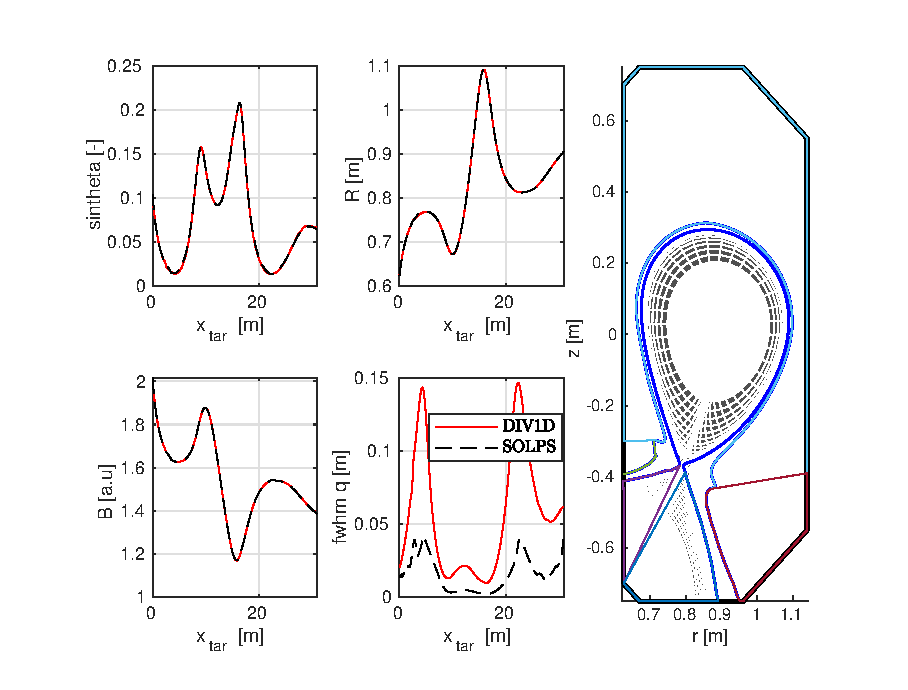
\includegraphics[width=\linewidth]{div1d_geometry.eps}
    \caption{The DIV1D geometry with on the left the magnetic field (B) and pitch angle (sintheta) followed by the radial coordinate (R) and width of the heat flux channel (fwhm q). Settings for DIV1D are based on SOLPS-ITER but the width is scaled to match plasma profiles in the SOL. On the right one can see the poloidal projection, using radial and vertical coordinates with associated normal vector to project the width of the SOL.}
    \label{fig:div1d-geometry}
\end{figure*}

\subsection{Boundary Conditions}

Each of these equations requires boundary conditions at the target/stagnation/X-point $x=0$ and at the (second) target $x=L$, where $L$ is the given length of the flux tube. At the stagnation point all fluxes are set to zero. At the X-point we use the following boundary conditions:
the plasma density at the X-point is given: $n(x=0) = n_{\rm X}$; the plasma momentum flux at the X-point assumed to be constant; the parallel heat flux at the X-point is given:  $q_\parallel(x=0) = q_{\parallel,\rm X}$; and finally, the neutral particle density is assumed to have zero gradient.

The boundary conditions at the target(s) are given by the usual sheath boundary conditions assuming that density and temperature are constant across the sheath, while the plasma particle flux and momentum are given by the Bohm condition, $\Gamma_n(x=L) \ge n c_{\rm s}$ and  where $c_{\rm s} = \sqrt{2eT/m}$ is the plasma sound speed, and the the heat flux on the target is given by the sheath heat transmission factor $\gamma$ which must be specified at input:
\begin{equation}\label{sheath_heat_transmission}
    q_\parallel(x=L) = \gamma n e T c_{\rm s}.
\end{equation}
The neutral particle flux coming from the target is determined by the recycling coefficient $R$ and a redistribution fraction $f_r$ given no input, i.e. $\Gamma_{\rm neutral}(x=0,x=L) = - R (1 - f_r) \Gamma_n(x=0,x=L)$.
Note that when $R=1$ and $f_r=0$ the total number of particles should be conserved requiring a zero plasma inflow velocity at the X-point in case of a steady state solution.


\subsection{Sources and Sinks}

The various sources and sinks are determined mostly by atomic processes like charge exchange, ionization, excitation, and recombination. In addition a neutral particle loss term can be specified in terms of an average residence time for the neutral in the flux tube to account for cross field neutral particle transport losses. For the plasma density the sources and sinks are given by:
\begin{equation}\label{particle_source}
    S_i=+n n_{\mathrm{n}}\left\langle\sigma_{\mathrm{ion}} v\right\rangle-n^2\left\langle\sigma_{\mathrm{rec}} v\right\rangle  - nn_m\langle\sigma v \rangle_{MAR} + nn_m\langle\sigma v \rangle_{MAI} 
\end{equation}

Because the neutral particle momentum is neglected there is no momentum source, while the momentum sinks are induced by:
\begin{equation}
\begin{aligned}
     S_{\rm mom} = & \; -(mv_\parallel-m_av_a)n n_a \langle\sigma_{\rm{cx}}v\rangle \\
     &-m_a(v_\parallel-v_a)nn_a\langle\sigma_m v\rangle(E_{rel}) \\
     &-m_av_\parallel n^2\left\langle\sigma_{\mathrm{rec}} v\right\rangle+v_am_a\langle \sigma_{ion}v\rangle \\
     &- m_a v_\parallel nn_m(\langle\sigma_{cx,m} v \rangle+\langle\sigma_{da} v \rangle +\langle\sigma_{mm} v\rangle(E_{rel,m})) ,
\end{aligned}
\label{eq:momentum_source}
\end{equation}
    where 
\begin{equation}
    E_{rel} = \frac{m_a(v_\parallel-v_a)^2}{2e}
\end{equation}
and
\begin{equation}
    E_{rel,m} = \frac{m_mv_\parallel^2}{2e}
\end{equation}

The energy balance contains both heat sinks and sources associated with charge exchange, hydrogenic ionization, and excitation, radiative and three-body recombination as well as impurity radiation
\begin{equation}\label{energy_source}
\begin{split}
    Q = &-n n_a \langle\sigma_{\rm cx} v\rangle e (1.5T - E_{a})  - 3 neT (n\langle\sigma_{\rm rec} v\rangle + n_m\langle\sigma v \rangle_{MAR}) \\
        &+ (\frac{1}{2} n m v^2_\parallel n_a +e E_a n n_a) \langle\sigma_{\rm ion} v\rangle +\frac{1}{2} n m v_{\|}^2 n_m\langle\sigma v\rangle_{MAI}\\
        &- n n_a eE_{\rm ion} \langle \sigma_{\rm ion} v\rangle - n n_a \langle eE_{\rm exc} \sigma_{\rm exc} v\rangle \\
        &-nn_m(eE_{ion,m}\langle \sigma_{ion,m} v\rangle + eE_{d,m} \langle \sigma_{d}v\rangle+eE_{cx,m}\langle \sigma_{cx,m}v\rangle) \\
        &-nn_me(\langle E_{rad,m}\sigma_{rad,m}v\rangle+eE_{da} \langle \sigma_{da}v\rangle) \\
        &+ n^2 \;eE_{\rm ion} \langle \sigma_{\rm rec} v\rangle - n^2 \;e\langle E_{\rm rad} \sigma_{\rm rec} v\rangle \\
        &+ Q_{di}+Q_{dr}+Q_{d,\mathrm{D_2^+}} + Q_{cx}^- + Q_{ion}^- \\
        &- n^2 \xi_Z L_Z(T)
\end{split}
\end{equation}
where the first line represents the losses to the neutrals (with energy $E_{\rm n}=1.5T_{\rm n}$) due to charge exchange and recombination and the second line is a source term from the neutrals that comes from ionization of (assumed momentum less) neutrals. The third line comes from ionization and the associated excitation, where $E_{\rm ion} = 13.6$~eV is the ionization energy and $E_{\rm exc}$ is the energy loss per excitation. In practice these are typically combined into an effective energy loss per ionization (see the paragraph below on the implemented reaction rates). The fourth line represents the effective energy balance from three-body and radiative recombination. Finally, the last line $L_Z(T)$ is the radiative cooling rate of the impurity with concentration $\xi$ for the specified impurity.

What is a sink for the plasma density is a source for the neutral particles, while additional neutral particle sources are associated with gas puff, redistribution of recycled neutrals or a possible exchange with a neutral background, such that
\begin{equation}\label{neutral_source}
\begin{aligned}
        S_a=&-n n_{\mathrm{n}}\left\langle\sigma_{\mathrm{ion}} v\right\rangle +n^2\left\langle\sigma_{\mathrm{rec}} v\right\rangle \\
        & + nn_m(3\langle\sigma v \rangle_{MAR} + \langle\sigma v \rangle_{MAI}^* + 2\langle\sigma v \rangle_{MAD}) \\
        &+ nn_m\langle\sigma_{d,m} v\rangle
        \\
        &+ S_{\rm puff} + S_{nn}^{\rm div} + S_{nn}^{\rm cor} 
\end{aligned}
\end{equation}
where 
\begin{equation}
    S_{nn}^{div} = - \frac{n_a-n_{b,a}}{\tau_a\lambda},
\end{equation}
and 
\begin{equation}
    S_{nn}^{cor} = - (1-f_{ion})\frac{n_a-n_{b,a}}{\tau_a\lambda}.
\end{equation}
where $S_{\rm puff}$ is a neutral particle source from an additional gas puff, and $S^{\rm cor/div}_{nn}$ accounts for neutral sources related to transport with external domains in the core and divertor scrape-off layer, denoted by superscripts. When a finite background neutral density $n_b$ is specified this term represents the exchange of neutrals in the leg with these background neutrals. The atomic rates for charge exchange, recombination, ionization, and excitation as used in the code as given in a later paragraph where also the impurity radiative cooling rates are be given.

\noindent The atom momentum balance source term is as follows
\begin{equation}
\begin{aligned}
     S_{\rm mom,a} = & \; (mv_\parallel-m_av_a)n n_a \langle\sigma_{\rm{cx}}v\rangle \\
     &+m_a(v_\parallel-v_a)nn_a\langle\sigma_m v\rangle(E_{rel}) \\
     &+v_\parallel n^2\left\langle\sigma_{\mathrm{rec}} v\right\rangle -v_am_a\langle \sigma_{ion}v\rangle  \\
     & +  m_a v_\parallel nn_m(\langle\sigma_{cx,m} v \rangle + \langle\sigma_{da} v \rangle) \\
     &-v_am_a\frac{n_a}{\tau_a\lambda} \\
\end{aligned}
\label{eq:S_mom,a}
\end{equation}
representing a mirror for the ion momentum balance and including losses for atoms that leave the scrape-off layer.
\noindent 

\noindent The molecule balance source term is as follows
\begin{equation}
    \begin{aligned}
    S_m =& -nn_m\left(\langle\sigma_{cx,m} v\rangle + \langle\sigma_{ion,m} v\rangle + \langle\sigma_{da} v\rangle + nn_m\langle\sigma_{d} v\rangle \right) \\
    &+ S_{puff,m}+S^{div}_{mm}+S^{cor}_{mm},
    \end{aligned}
\end{equation}

where 
\begin{equation}
    S_{mm}^{div} = - \frac{n_m-n_{b,m}}{\tau_m\lambda},
\end{equation}

and 
\begin{equation}
    S_{mm}^{cor} = - (1-f_{ion})\frac{n_m-n_{b,m}}{\tau_m\lambda}.
\end{equation}
Similar to the atomic balance.
%  The flux of external neutrals into the scrape-off layer is determined as 
% \begin{equation}
% \begin{aligned}
%          \Gamma^{\vdash}_{nn} &=  (n_{\rm b}-n_{\rm n})A_{\rm extern} v_{\rm ex}   \quad \mathrm{[s^{-1}]},
%      \end{aligned} % \cdot \lambda_q
%  \end{equation}
% where the cross-tube neutral flux $\Gamma_{\rm nn}^{\vdash}$ follows from the difference between external gas density $n_{\rm nb}$ and neutral SOL density $n_{n}$, multiplied with the external area $A_{\rm extern}$ and an exchange velocity $v_{\rm ex}$. Here it is noted that $v_{\rm ex}$ replaces the neutral exchange time $\tau_{\rm ex}$ in \cite{derks2022} and that the external neutral gas density $n_{\rm b}$ for the divertor and core region can be set independently to mimic density differences caused by baffles. 

% The cross-sol neutral flux enters the divertor scrape-off layer from both the private flux region (PFR) and common flux region (CFR). As such the divertor-SOL neutral source is determined by:
% \begin{equation}
%      S^{\rm div}_{nn} = (\Gamma^{\vdash,PFR}_{nn} + \Gamma^{\vdash,CFR}_{nn})  \cdot V^{-1}  \quad \mathrm{[s^{-1}m^{-3}]},
% \end{equation}
% where fluxes from the PFR and CFR are divided by the volumes $V$. For the neutral flux into the core-SOL it is noted that a large fraction $f_{\rm core,ion}$ can propagate into the core before being ionized, reducing the neutral source in the core-SOL as follows:
% \begin{equation}
%         S^{\rm core}_{nn} = \Gamma^\vdash_{nn}(1-f_{\rm core,ion})/V  \quad \mathrm{[s^{-1}m^{-3}]}.
% \end{equation}

For simulations with a core scrape-off layer the fluxes established at the X-point originate from the core and neutral reservoirs external to the scrape-off layer. The plasma sources that originate from the core are calculated using the total core heat and ion fluxes $\Gamma_{\rm core}~\mathrm{[ s^{-1}]}$ and $Q_{\rm core}~\mathrm{[J s^{-1}]}$, respectively. These fluxes are multiplied with a normalized distribution.
This core source distribution is calculated as follows
\begin{equation}
    d(x) = (1 - ([x-x_{\rm center}]/L_{\rm core})^2)^{\alpha} \cdot A
\end{equation}
and normalized such that the integral equals unity. The profile shaping parameter $\alpha$ can be used to shape the distribution and create peaked or flat profiles symmetric arround $x_{\rm center}$, enabling varying flux distributions over the seperatrix due to different (neoclassical or anomalous) transport phenomena. $x_{\rm center}$ equals zero (one leg) or $L_{\rm core}/2$ (two legs). Multiplication with the area $A$ in the normalized distribution allows direct division with the volume to obtain volumetric sources for heat and particles (respectively $S_{\rm ene}^{\rm core} $ and $S_{n}^{\rm core}$) as follows:
\begin{equation}
\begin{aligned}
    S_{\rm ene}^{\rm core} = \Gamma_{{\rm ene}}^{\rm core} \cdot d^{ene} \cdot  V^{-1} \\
    S_{n}^{\rm core} = \Gamma_{n}^{\rm core} \cdot d^n \cdot  V^{-1} 
    \end{aligned}
\end{equation}
where the flux distributions are equal for particles and heat. The sink of ionized particles caused by fluxes into the far-sol should be left out (although this channel is numerically available). Firstly because these fluxes are partly redirected into the divertor. Secondly to reduce the number of free parameters as the particle balance also depends on the core-ionization fraction $f_{\rm core,ion}$. The sources are considered in the main equations of DIV1D according to their subscripts, e.g. $S_{\rm ene}^{\rm core}$ is added tot the right hand side of the energy balance.

\subsection{External reservoirs}
A short explanation of the setup of the reservoirs outside the scrape-off layer. There are 5 external reservoirs. The private flux region (1,5), divertor common flux regions (2,4) and core common flux region (3) with volumes ($\tt extern\_neutral\_volumes$). There can be fluxes between the external neutral reservoirs. These fluxes are defined clock-wise as: 2$\rightarrow$3, 3$\rightarrow$4,  5$\rightarrow$1 with external exchange times ($\tt extern\_neutral\_extimes(1:3)$), respectively. Fluxes that recycle at the target are redistributed using the redistributed fraction $f_{\rm red}$. This will distribute a fraction of the recycling target flux into external volumes 2,1,5,4. A poloidal target angle ($\tt pol\_target\_angle(1,2)$, 0-180) where for 0 all fluxes go to 1+4 and for 180 all fluxes go to 2+5. The fluxes between reservoir and scrape-off layer are directed into the scrape-off layer.

\subsection{Wall association}
The wall can be set to associate atoms into molecules.
The rate at which this happens is set as $tau_{wa}$, standing for wall association.

\begin{equation}
    \begin{aligned}
        \Gamma_w = \frac{1}{4}n^r_{atom} \cdot v 
        =  \frac{1}{4}n^r_{atom} \cdot \sqrt{\frac{2 e T^r_{atom}}{m}} ~\mathrm{[m^{-2} s^{-1}]} \\
        S_w = \Gamma_w \cdot A^r_w ~\mathrm{[ s^{-1}]} \\
        s^r_{mol} =\frac{1}{2} \left[ \frac{A^r_w}{ V^r} \cdot \frac{1}{4}n_{atom} \cdot \sqrt{\frac{2 e T^r_{atom}}{m}}\right]~\mathrm{[m^{-3} s^{-1}]}
    \end{aligned}
\end{equation}
Which adds as parameters to the DIV1D code the wall area $A^r_w~\mathrm{[m^2]}$ per reservoir and a neutral atom temperature $T^r_{atom}~\mathrm{[eV]}$ per reservoir. To simplify the code, the conversion speed $\eta_{wall,association}= \frac{1}{4} \cdot v 
        =  \frac{1}{4}\cdot\sqrt{\frac{2 e T^r_{atom}}{m}}~\mathrm{[m/s]}$ is set directly instead of the neutral temperature. 
        So there is no neutral-atom temperature but rather a wall association speed set for the reservoirs. 

        % note that this velocity is the same as the exchange  velocity with the SOL.
        % add probability of association as free parameter.

% \subsection{Target recycling}
% The target recycling in DIV1D can be set with .. \textbf{add description of neutral target recycling values}

% \subsection{Radial power losses}
% The power losses in the radial direction can be modelled through a radial power loss factor. Although one should be cautious when using this together with flux expansion as  they have similar effects on the power balance.
% To simulate this effect, DIV1D includes several versions of an effective radial loss term. The simplest version is
% \begin{equation}
% \label{constant_rad_losses}
% S_{\perp}=-\eta_{\perp}\frac{q_\parallel}{L}
% \end{equation}

% where $S_{\perp}$ denotes the radial power sink, and $\eta_{\perp}$ is the fraction of the upstream heat flux that is lost over the length of the flux tube due to radial losses. A slightly more advanced version of these losses is

% \begin{equation}
% S_\perp(x)=-\frac{\eta_{\perp}q_{\parallel}}{\sqrt{2\pi(\mathrm{\Delta}x)^2}}
% \mathrm{exp}{-\frac{1}{2}\left(\frac{x-x_0}{\mathrm{\Delta}x}\right)^2}
% \end{equation}

% where losses are no longer incurred equally over the flux tube, but are instead peaked at $x_0$ with a typical width of $\mathrm{\Delta}x$ around it. Note that the prefactor is calculated analytically in the code to make sure that the total losses always amount to $-\eta_{\perp}\times q_{\parallel}$. A comparison of either loss profile show that the target parameters are rather indifferent to the choice of loss profile.\\

% Finally, a heat-flux-dependent variant is also included as

% \begin{equation}
% S_{\perp}=-\eta_{\perp}\frac{q_\parallel(x)}{L}
% \end{equation}

% which is crucially different from~\ref{constant_rad_losses} in that it takes into account the local heat flux in each grid cell rather than the upstream heat flux. As a result $\eta_{\perp}$ no longer reflects the total fraction of the upstream heat flux that is lost.\\

% Four input parameters exist which the user can employ to shape the radial losses to his or her desire. These are:
% radial\_loss\_factor ($\eta_{\perp}$),
% radial\_loss\_gaussian (choice of loss profile),
% radial\_loss\_width ($\mathrm{\Delta}x$), and
% radial\_loss\_location ($x_0$). See table~2.



\section{Atomic Rates}\label{rates}

A number of different options is available to calculate the atomic rates. For each of the rates a number of options is provided for different expressions that have been used in the literature. These include approximate formulas which are used amongts others in the SD1D code \cite{SD1D} of which the origin is however not always fully clear. The to our knowledge more accurate rates are obtained from the AMJUEL data base that is also being used for the EIRENE neutral particle Monte Carlo code and which can be found at the web site of the code \cite{EIRENE}. By default the rates from the AMJUEL data base are selected.


\subsection{Charge Exchange}

The default option uses the charge exchange rate as specified in section 2.19 reaction 3.1.8 of the AMJUEL data base for the total charge exchange rate of Hydrogen~\cite{EIRENE}. This uses a fit function of the form
\begin{equation}\label{charge_exchange_AMJUEL}
    \langle\sigma_{\rm cx} v\rangle = 10^{-6} \exp\left( \sum_{i=0}^8 b_i (\ln T)^i \right)  {\rm m}^3/{\rm s}
\end{equation}
with the fitting constants $b_i$ defined by
\begin{small}\begin{verbatim}
   b0 -1.850280000000E+01    b1  3.708409000000E-01    b2  7.949876000000E-03
   b3 -6.143769000000E-04    b4 -4.698969000000E-04    b5 -4.096807000000E-04
   b6  1.440382000000E-04    b7 -1.514243000000E-05    b8  5.122435000000E-07
\end{verbatim}\end{small}
Note that the factor $10^{-6}$ stems from the use of the units ${\rm cm}^3/{\rm s}$ for the reaction rates in AMJUEL.

In order to allow comparisons with models from other authors a number of alternative options are provided for the caclculations of the reaction rates. This includes the charge exchange rate as implemented in SD1D originating from the work by Havlickova \cite{havlickova2013} which is given by \cite{SD1D}
\begin{equation}\label{charge_exchange_SD1D}
    \langle\sigma_{\rm cx} v\rangle = \begin{cases} 1.0 \times 10^{-14} {\rm m}^3/{\rm s}             & \mbox{for } T \le 1 {\rm eV} \\
                                        1.0 \times 10^{-14} T^{1/3} {\rm m}^3/{\rm s} & \mbox{for } T >   1 {\rm eV}. \end{cases}
\end{equation}
This option is selected by setting {\tt case\_cx = "Havlickova"}.

Another expression that has been used for example in the work by Nakazawa et al. \cite{nakazawa2000}, comes from Table 3 of the report by Freeman and Jones \cite{freeman1974} in which case the charge exchange rate is given by a fit function of the same form as above
\begin{equation}\label{charge_exchange_FJ}
    \langle\sigma_{\rm cx} v\rangle = 10^{-6} \exp\left( \sum_{i=0}^8 b_i (\ln T)^i \right)  {\rm m}^3/{\rm s}
\end{equation}
with fitting coefficients $b_i$ now given as
\begin{small}\begin{verbatim}
   b0 -1.841757E+01  b1  5.282950E-01  b2 -2.200477E-01
   b3  9.750192E-02  b4 -1.749183E-02  b5  4.954296E-04
   b6  2.174910E-04  b7 -2.530206E-05  b8  8.230751E-07
\end{verbatim}\end{small}
This option is selected by setting {\tt case\_cx = "Freeman"}. The validity range of this fit is indicated as 1 to $10^5$~eV.

Charge exchange rates for the Hydrogen isotopes like Deuterium and Tritium are obtained by the same expressions given above, but using a rescaled temperature multiplied with the factor $m_p/m_i$, i.e. the ratio of the proton mass over the mass of the Deuterium or Tritium ion, respectively.


\subsection{Ionization}
The default option for calculation of the ionization rate is also obtained from the AMJUEL data base, which provides an effective ionization rate as calculated using a double fit function
\begin{equation}\label{ionization_AMJUEL}
    \langle\sigma_{\rm ion} v\rangle = 10^{-6} \exp\left( \sum_{i=0}^8\sum_{j=0}^8 \alpha_{ij} (\ln \bar n)^j (\ln T)^i \right)  {\rm m}^3/{\rm s}
\end{equation}
where the density is normalized as $\bar n \equiv n / 10^{14}$ and the fitting coefficients $\alpha_{ij}$ are given in section 4.3 reaction 2.1.5 of the AMJUEL document for the case of the total ionization rate (including all excited states of the neutral hydrogen atoms)
\begin{small}\begin{verbatim}
        n-Index:     0                     1                     2
  T-Index:
        0   -3.248025330340D+01   -5.440669186583D-02    9.048888225109D-02
        1    1.425332391510D+01   -3.594347160760D-02   -2.014729121556D-02
        2   -6.632235026785D+00    9.255558353174D-02   -5.580210154625D-03
        3    2.059544135448D+00   -7.562462086943D-02    1.519595967433D-02
        4   -4.425370331410D-01    2.882634019199D-02   -7.285771485050D-03
        5    6.309381861496D-02   -5.788686535780D-03    1.507382955250D-03
        6   -5.620091829261D-03    6.329105568040D-04   -1.527777697951D-04
        7    2.812016578355D-04   -3.564132950345D-05    7.222726811078D-06
        8   -6.011143453374D-06    8.089651265488D-07   -1.186212683668D-07

        n-Index:     3                     4                     5
  T-Index:
        0   -4.054078993576D-02    8.976513750477D-03   -1.060334011186D-03
        1    1.039773615730D-02   -1.771792153042D-03    1.237467264294D-04
        2   -5.902218748238D-03    1.295609806553D-03   -1.056721622588D-04
        3    5.803498098354D-04   -3.527285012725D-04    3.201533740322D-05
        4    4.643389885987D-04    1.145700685235D-06    8.493662724988D-07
        5   -1.201550548662D-04    6.574487543511D-06   -9.678782818849D-07
        6    8.270124691336D-06    3.224101773605D-08    4.377402649057D-08
        7    1.433018694347D-07   -1.097431215601D-07    7.789031791949D-09
        8   -2.381080756307D-08    6.271173694534D-09   -5.483010244930D-10

        n-Index:     6                     7                     8
  T-Index:
        0    6.846238436472D-05   -2.242955329604D-06    2.890437688072D-08
        1   -3.130184159149D-06   -3.051994601527D-08    1.888148175469D-09
        2    4.646310029498D-06   -1.479612391848D-07    2.852251258320D-09
        3   -1.835196889733D-06    9.474014343303D-08   -2.342505583774D-09
        4   -1.001032516512D-08   -1.476839184318D-08    6.047700368169D-10
        5    5.176265845225D-08    1.291551676860D-09   -9.685157340473D-11
        6   -2.622921686955D-09   -2.259663431436D-10    1.161438990709D-11
        7   -4.197728680251D-10    3.032260338723D-11   -8.911076930014D-13
        8    3.064611702159D-11   -1.355903284487D-12    2.935080031599D-14
T1MIN =   0.10000D 00 EV
T1MAX =   2.00000D 04 EV
N2MIN =   1.00000D 08 1/CM3
N2MAX =   1.00000D 16 1/CM3
\end{verbatim}\end{small}

One alternative option is again provided in the form of the ionization rate as implemented in SD1D originating from the work by Havlickova \cite{havlickova2013}. It is slightly modified to remove the discontinuity at 20~eV and is given by \cite{SD1D}
\begin{equation}\label{ionization_SD1D}
    \langle\sigma_{\rm ion} v\rangle = \begin{cases} 7.638 \times 10^{-21} {\rm m}^3/{\rm s}             & \mbox{for } T \le 1 {\rm eV} \\
                                        10^{-6.0d+0} T^{-2.987} 10^{-15.72 \exp(-\log_{10}T) + 1.603*exp(-\log_{10}^2T)} {\rm m}^3/{\rm s} & \mbox{for } 1 {\rm eV} < T \le 20 {\rm eV} \\
                                        5.875 \times 10^{-12} T^{-0.5151} 10^{-2.563/\log_{10}T} {\rm m}^3/{\rm s}. \end{cases}
\end{equation}
This option is selected by setting {\tt case\_ion = "Havlickova"}

A further option again comes from the work of Nakazawa et al.~\cite{nakazawa2000} who use the ionization rate given in Table 3 of the report by Freeman and Jones~\cite{freeman1974}. They provide a fit to the electron impact ionization given by
\begin{equation}\label{ionization_FJ}
    \langle\sigma_{\rm ion} v\rangle = 10^{-6} \exp\left( \sum_{i=0}^6 b_i (\ln T)^i \right)  {\rm m}^3/{\rm s}
\end{equation}
with fitting coefficients $b_i$ given by
\begin{small}\begin{verbatim}
   b0 -0.3173850E+02  b1  0.1143818E+02  b2 -0.3833998E+01
   b3  0.7046692E+00  b4 -0.7431486E-01  b5  0.4153749E-02
   b6 -0.9486967E-04
\end{verbatim}\end{small}
This option is selected by setting {\tt case\_ion = "Freeman"}


\subsection{Excitation and ionization energy losses}

By default, the sum of energy losses from ionization and excitation is obtained from the AMJUEL data base, which provides an effective excitation rate in terms of an averaged effective energy loss per ionization. This is calculated from a fit function of the same form as defined above for the ionization rate (\ref{ionization_AMJUEL}), i.e.
\begin{equation}
  \langle E_{\rm ion} \sigma_{\rm ion} v\rangle + \langle E_{\rm exc} \sigma_{\rm exc} v\rangle =  10^{-6} \exp\left( \sum_{i=0}^8\sum_{j=0}^8 \alpha_{{\rm exc,} ij} (\ln \bar n)^j (\ln T)^i \right)  {\rm eV} {\rm m}^3/{\rm s}
\end{equation}
with the coefficients $\alpha_{{\rm exc,} ij}$ as tabulated in section 10.2 for reaction 2.5.1 of the AMJUEL document for the case of the total energy loss rate associated with Hydrogen ionization and excitation radiation:
\begin{small}\begin{verbatim}
        n-Index:     0                     1                     2
  T-Index:
        0   -2.497580168306D+01    1.081653961822D-03   -7.358936044605D-04
        1    1.004448839974D+01   -3.189474633369D-03    2.510128351932D-03
        2   -4.867952931298D+00   -5.852267850690D-03    2.867458651322D-03
        3    1.689422238067D+00    7.744372210287D-03   -3.087364236497D-03
        4   -4.103532320100D-01   -3.622291213236D-03    1.327415215304D-03
        5    6.469718387357D-02    8.268567898126D-04   -2.830939623802D-04
        6   -6.215861314764D-03   -9.836595524255D-05    3.017296919092D-05
        7    3.289809895460D-04    5.845697922558D-06   -1.479323780613D-06
        8   -7.335808238917D-06   -1.367574486885D-07    2.423236476442D-08

        n-Index:     3                     4                     5
  T-Index:
        0    4.122398646951D-04   -1.408153300988D-04    2.469730836220D-05
        1   -7.707040988954D-04    1.031309578578D-04   -3.716939423005D-06
        2   -8.328668093987D-04    2.056134355492D-04   -3.301570807523D-05
        3    4.707676288420D-04   -5.508611815406D-05    7.305867762241D-06
        4   -1.424078519508D-04    3.307339563081D-06    5.256679519499D-09
        5    2.411848024960D-05    5.707984861100D-07   -1.016945693300D-07
        6   -1.474253805845D-06   -2.397868837417D-07    1.518743025531D-08
        7   -4.633029022577D-08    3.337390374041D-08   -1.770252084837D-09
        8    5.733871119707D-09   -1.512777532459D-09    8.733801272834D-11

        n-Index:     6                     7                     8
  T-Index:
        0   -2.212823709798D-06    9.648139704737D-08   -1.611904413846D-09
        1   -4.249704742353D-07    4.164960852522D-08   -9.893423877739D-10
        2    2.831739755462D-06   -1.164969298033D-07    1.785440278790D-09
        3   -6.000115718138D-07    2.045211951761D-08   -1.790312871690D-10
        4    7.597020291557D-10    1.799505288362D-09   -9.280890205774D-11
        5    3.517154874443D-09   -4.453195673947D-10    2.002478264932D-11
        6    4.149084521319D-10   -6.803200444549D-12   -1.151855939531D-12
        7   -5.289806153651D-11    3.864394776250D-12   -8.694978774411D-15
        8    7.196798841269D-13   -1.441033650378D-13    1.734769090475D-15
T1MIN =   0.10000D 00 EV
T1MAX =   2.00000D 04 EV
N2MIN =   1.00000D 08 1/CM3
N2MAX =   1.00000D 16 1/CM3
\end{verbatim}\end{small}


Energy losses from ionization and due to excitation radiation are accounted for either as an effective energy loss constant per ionization (typically $E_{eff,ion} = 30$~eV as in Nakazawa et al. \cite{nakazawa2000}) which can be specified at input er by an effective excitation rate which accounts for the temperature and density dependent total energy loss from ionization and excitation radiation. In the SD1D code the latter is given by a simple fit function as
\begin{equation}\label{excitation_SD1D}
    \langle\sigma_{\rm exc} v\rangle = {4.90 \times 10^{-13} \over 0.28 + Y} \exp(-Y) \sqrt{Y (1.0 + Y)} {\rm eV} {\rm m}^3/{\rm s},
\end{equation}
where $Y = 10.2 / \max( 1, T)$. Added to this is the 13.6~eV of energy loss per ionization.



\subsection{Recombination}

In their 1D code Nakazawa et al.~\cite{nakazawa2000} use a combination of the radiative recombination rate from Gordeev et al. plus the three body recombination rate given by Hinnov et al., where the former is given by the expression~\cite{gordeev1977}
\begin{equation}\label{radiative_recombination}
    \langle\sigma_{\rm rad.rec} v\rangle = 1.27 \times 10^{-19} {(13.6./T)^{1.5} \over (13.6/T) + 0.59} {\rm m}^3 / s,
\end{equation}
and the latter is expressed as~\cite{hinnov1962}
\begin{equation}\label{three_body_recombination}
    \langle\sigma_{\rm 3bodyrec} v\rangle = 5.6 \times 10^{-39} \; T^{-4.5} n {\rm m}^3 / s.
\end{equation}
This model is selected by setting {\tt case\_rec = "Nakazawa"}.

Otherwise, the recombination rate is used from the AMJUEL data providing the total effective recombination rate including 3 body recombination using again a fit function (\ref{ionization_AMJUEL}) as defined above for the ionization rate, now with the coefficients $\alpha_{{\rm rec,} ij}$ as tabulated in section 4.6 reaction 2.1.8 of the AMJUEL document:
\begin{small}\begin{verbatim}
        n-Index:     0                     1                     2
  T-Index:
        0   -2.858858570847D+01    2.068671746773D-02   -7.868331504755D-03
        1   -7.676413320499D-01    1.278006032590D-02   -1.870326896978D-02
        2    2.823851790251D-03   -1.907812518731D-03    1.121251125171D-02
        3   -1.062884273731D-02   -1.010719783828D-02    4.208412930611D-03
        4    1.582701550903D-03    2.794099401979D-03   -2.024796037098D-03
        5   -1.938012790522D-04    2.148453735781D-04    3.393285358049D-05
        6    6.041794354114D-06   -1.421502819671D-04    6.143879076080D-05
        7    1.742316850715D-06    1.595051038326D-05   -7.858419208668D-06
        8   -1.384927774988D-07   -5.664673433879D-07    2.886857762387D-07

        n-Index:     3                     4                     5
  T-Index:
        0    3.843362133859D-03   -7.411492158905D-04    9.273687892997D-05
        1    3.828555048890D-03   -3.627770385335D-04    4.401007253801D-07
        2   -3.711328186517D-03    6.617485083301D-04   -6.860774445002D-05
        3   -1.005744410540D-03    1.013652422369D-04   -2.044691594727D-06
        4    6.250304936976D-04   -9.224891301052D-05    7.546853961575D-06
        5   -3.746423753955D-05    7.509176112468D-06   -8.688365258514D-07
        6   -1.232549226121D-05    1.394562183496D-06   -6.434833988001D-08
        7    1.774935420144D-06   -2.187584251561D-07    1.327090702659D-08
        8   -6.591743182569D-08    8.008790343319D-09   -4.805837071646D-10

        n-Index:     6                     7                     8
  T-Index:
        0   -7.063529824805D-06    3.026539277057D-07   -5.373940838104D-09
        1    1.932701779173D-06   -1.176872895577D-07    2.215851843121D-09
        2    4.508046989099D-06   -1.723423509284D-07    2.805361431741D-09
        3   -4.431181498017D-07    3.457903389784D-08   -7.374639775683D-10
        4   -3.682709551169D-07    1.035928615391D-08   -1.325312585168D-10
        5    7.144767938783D-08   -3.367897014044D-09    6.250111099227D-11
        6   -2.746804724917D-09    3.564291012995D-10   -8.551708197610D-12
        7   -1.386720240985D-10   -1.946206688519D-11    5.745422385081D-13
        8    6.459706573699D-12    5.510729582791D-13   -1.680871303639D-14
T1MIN =   0.10000D 00 EV
T1MAX =   2.00000D 04 EV
N2MIN =   1.00000D 08 1/CM3
N2MAX =   1.00000D 16 1/CM3
\end{verbatim}\end{small}

When the default option is selected to use the data from AMJUEL also the energy lost and gained by the electrons due to radiative and three-body recombination is taken into account. In this case the effective electron cooling rate from the associated processes is obtained from the fit specified in AMJUEL section 10.4 for the recombination reaction and taking into account the 13.6~eV potential enrgy gain per effective recombination event, i.e.
\begin{equation}
  \langle E_{\rm el} \sigma_{\rm rec} v\rangle =  10^{-6} \exp\left( \sum_{i=0}^8\sum_{j=0}^8 \alpha_{{\rm rec el,} ij} (\ln \bar n)^j (\ln T)^i \right) - 13.6 \langle\sigma_{\rm rec} v\rangle  {\rm eV} {\rm m}^3/{\rm s}
\end{equation}
where the effective recombination rate $\langle\sigma_{\rm rec} v\rangle$ is obtained from the fit specified before and the coefficients $\alpha_{{\rm rec el,} ij}$ of the current fit are given by
\begin{small}\begin{verbatim}

        E-Index:     0                     1                     2
  T-Index:
        0   -2.592450349909D+01    1.222097271874D-02    4.278499401907D-05
        1   -7.290670236493D-01   -1.540323930666D-02   -3.406093779190D-03
        2    2.363925869096D-02    1.164453346305D-02   -5.845209334594D-03
        3    3.645333930947D-03   -1.005820792983D-03    6.956352274249D-04
        4    1.594184648757D-03   -1.582238007548D-05    4.073695619272D-04
        5   -1.216668033378D-03   -3.503070140126D-04    1.043500296633D-04
        6    2.376115895241D-04    1.172709777146D-04   -6.695182045674D-05
        7   -1.930977636766D-05   -1.318401491304D-05    8.848025453481D-06
        8    5.599257775146D-07    4.977823319311D-07   -3.615013823092D-07

        E-Index:     3                     4                     5
  T-Index:
        0    1.943967743593D-03   -7.123474602102D-04    1.303523395892D-04
        1    1.532243431817D-03   -4.658423772784D-04    5.972448753445D-05
        2    2.854145868307D-03   -5.077485291132D-04    4.211106637742D-05
        3   -9.305056373739D-04    2.584896294384D-04   -3.294643898894D-05
        4   -9.379169243859D-05    1.490890502214D-06    2.245292872209D-06
        5    9.536162767321D-06   -6.908681884097D-06    8.232019008169D-07
        6    1.188184006210D-05   -4.381514364966D-07   -6.936267173079D-08
        7   -2.072370711390D-06    2.055919993599D-07   -7.489632654212D-09
        8    9.466989306497D-08   -1.146485227699D-08    6.772338917155D-10

        E-Index:     6                     7                     8
  T-Index:
        0   -1.186560752561D-05    5.334455630031D-07   -9.349857887253D-09
        1   -4.070843294052D-06    1.378709880644D-07   -1.818079729166D-09
        2   -1.251436618314D-06   -1.626555745259D-08    1.073458810743D-09
        3    2.112924018518D-06   -6.544682842175D-08    7.810293075700D-10
        4   -3.150901014513D-07    1.631965635818D-08   -2.984093025695D-10
        5   -2.905331051259D-08   -3.169038517749D-10    2.442765766167D-11
        6    6.592249255001D-09   -1.778887958831D-10    1.160762106747D-12
        7   -7.073797030749D-11    1.047087505147D-11   -1.877446271350D-13
        8   -1.776496344763D-11    7.199195061382D-14    3.929300283002D-15
T1MIN =   0.10000D 00 EV
T1MAX =   2.00000D 04 EV
N2MIN =   1.00000D 08 1/CM3
N2MAX =   1.00000D 16 1/CM3

  Max. rel. Error:   0.930E+01 %
  Mean rel. Error:   0.127E+01 %
\end{verbatim}\end{small}

\section{Molecular activated processes in DIV1D}
\label{sec: MA rates}
\textbf{Here we should add the AMJUEL tables that are implemented}

The molecular activated reaction rates used in DIV1D are given here: 


\begin{equation}
    \langle\sigma v\rangle_{MAR} = \frac{\langle\sigma_{cx,m} v\rangle +  \langle\sigma_{ion,m} v\rangle}{ \langle\sigma_{dr} v\rangle +  \langle\sigma_{d,\mathrm{D}_2^+} v\rangle  +  \langle\sigma_{di} v\rangle }\langle\sigma_{dr} v\rangle f_{cx}
\end{equation}

\begin{equation}
    \langle\sigma v\rangle_{MAD} = \frac{\langle\sigma_{cx,m} v\rangle +  \langle\sigma_{ion,m} v\rangle}{ \langle\sigma_{dr} v\rangle +  \langle\sigma_{d,\mathrm{D}_2^+} v\rangle  +  \langle\sigma_{di} v\rangle }(\langle\sigma_{d,\mathrm{D}_2^+}v\rangle f_{cx} + (1-f_{cx})\langle\sigma_{dr} v\rangle)
\end{equation}

\begin{equation}
    \langle\sigma v\rangle_{MAI} = \frac{\langle\sigma_{cx,m} v\rangle +  \langle\sigma_{ion,m} v\rangle}{ \langle\sigma_{dr} v\rangle +  \langle\sigma_{d,\mathrm{D}_2^+} v\rangle  +  \langle\sigma_{di} v\rangle }(\langle\sigma_{di} v\rangle f_{cx} + (1-f_{cx})(\langle\sigma_{d,\mathrm{D}_2^+}v\rangle+ 2\langle\sigma_{di} v\rangle))
\end{equation}

\begin{equation}
    \langle\sigma v\rangle_{MAI}^* = \frac{\langle\sigma_{cx,m} v\rangle +  \langle\sigma_{ion,m} v\rangle}{ \langle\sigma_{dr} v\rangle +  \langle\sigma_{d,\mathrm{D}_2^+} v\rangle  +  \langle\sigma_{di} v\rangle }(\langle\sigma_{di} v\rangle f_{cx} + (1-f_{cx})\langle\sigma_{d,\mathrm{D}_2^+}v\rangle)
\end{equation}

\begin{equation}
    f_{cx} = \frac{\langle\sigma_{cx,m} v\rangle}{\langle\sigma_{cx,m} v\rangle + \langle\sigma_{ion,m} v\rangle}
\end{equation}

Reaction rates for MAR and MAD through D$^-$: 
\begin{equation}
    \langle\sigma v\rangle_{MAR}^- = \frac{\langle\sigma_{da} v\rangle}{  \langle \sigma_{cx,\mathrm{D}^-} v\rangle  +  \langle \sigma_{ion,\mathrm{D}^-} v\rangle}\langle \sigma_{cx,\mathrm{D}^-} v\rangle
\end{equation}

\begin{equation}
    \langle\sigma v\rangle_{MAD}^- = \frac{\langle\sigma_{da} v\rangle}{  \langle \sigma_{cx,\mathrm{D}^-} v\rangle  +  \langle \sigma_{ion,\mathrm{D}^-} v\rangle}\langle \sigma_{ion,\mathrm{D}^-} v\rangle
\end{equation}

Energy loss rates through reactions with D$_2^+$ and $D^-$. 

\begin{equation}
    Q_{d,\mathrm{D}_2^+} = -nn_{\mathrm{D_2^+}}eD_0(\mathrm{D}_2^+)\langle\sigma_{d,\mathrm{D}_2^+}v\rangle
\end{equation}

\begin{equation}
    Q_{di} = -nn_{\mathrm{D_2^+}}e\left[D_0(\mathrm{D}_2^+)+E_{ion}\right]\langle\sigma_{di}v\rangle
\end{equation}

\begin{equation}
    Q_{dr} = -nn_{\mathrm{D_2^+}}e\left[D_0(\mathrm{D}_2^+)-E_{ion}\right]\langle\sigma_{dr}v\rangle
    \label{eq:Q_dr}
\end{equation}

In \eqref{eq:Q_dr}, three-body recombination is assumed to be dominant. The following are the energy losses through reactions with D$^-$. 

\begin{equation}
    Q_{cx}^- = -nn_{\mathrm{D}^-}eE_{b,\mathrm{D}^-}\langle\sigma_{cx, \mathrm{D}^-}v\rangle
    \label{eq:Qcxmin}
\end{equation}

\begin{equation}
    Q_{ion}^- = -nn_{\mathrm{D}^-}e\left[E_{b,\mathrm{D}^-} + E_{ion}\right]\langle\sigma_{ion, \mathrm{D}^-}v\rangle
    \label{eq:Qionmin}
\end{equation}

Ionic densities: 
\begin{equation}
    n_{\mathrm{D}_2^+} = n_m  \frac{\langle\sigma_{cx,m} v\rangle +  \langle\sigma_{ion,m} v\rangle}{ \langle\sigma_{dr} v\rangle +  \langle\sigma_{d,\mathrm{D}_2^+} v\rangle  +  \langle\sigma_{di} v\rangle }
\end{equation}

\begin{equation}
    n_{\mathrm{D}^-} = n_m \frac{\langle\sigma_{da} v\rangle}{  \langle \sigma_{cx,\mathrm{D}^-} v\rangle  +  \langle \sigma_{ion,\mathrm{D}^-} v\rangle}
\end{equation}


\newpage
\section{Table of collisional-radiative processes in DIV1D}
\label{sec: Appendix reaction rates table}
This section contains a table of all the collisional-radiative processes included in DIV1D, including reaction formula and rate constants. 

\begin{longtable}[c]{|l|l|l|}
\hline
Reaction             & Formula & Rate constant  \\
\hline
 & &\\
Electron impact ionization  & $e+\mathrm{D}\rightarrow2e+\mathrm{D}^+$ & $\langle \sigma_{ion} v\rangle $\\
 & &\\
Charge exchange  & $\mathrm{D}^++\mathrm{D}\rightarrow\mathrm{D}+\mathrm{D}^+$ & $\langle \sigma_{cx} v\rangle $ \\
 & & \\
Electron ion recombination (radiative + three-body)  & $e+\mathrm{D}^+\rightarrow \mathrm{D}$ & $\langle \sigma_{rec} v\rangle $ \\
 & &\\
Electron ion recombination radiative power loss & $e+\mathrm{D}^+\rightarrow \mathrm{D} + \hbar\omega$ & $\langle E_{rad} \sigma_{rec} v\rangle $ \\
 & &\\
Electron impact excitation + radiative decay & $e+\mathrm{D}\rightarrow e + \mathrm{D}^* \rightarrow e+\mathrm{D}+ \hbar\omega$ & $\langle E_{exc} \sigma_{exc} v\rangle $\\
 & &\\
Dissociative attachment & $e+\text{D}_2\rightarrow \text{D}^-+\text{D}$ & $\langle \sigma_{da} v\rangle $   \\
 & &\\
Molecular ionization & $e+\text{D}_2\rightarrow 2e+\text{D}_2^+$ & $\langle \sigma_{ion, m} v\rangle $\\
 & &\\
Electron impact dissociation & $e+\text{D}_2(n,\nu)\rightarrow e+2\text{D}$ & $\langle \sigma_{d} v\rangle $\\
 & &\\
Molecular charge exchange & $\text{D}^++\text{D}_2\rightarrow \text{D} + \text{D}_2^+$ & $\langle \sigma_{cx,m} v\rangle $\\
 & &\\
Dissociative recombination & $e+\text{D}_2^+\rightarrow 2\text{D}$ & $\langle \sigma_{dr} v\rangle $  \\
 & &\\
Electron impact dissociation (with D$_2^+$) &  $e+\text{D}_2^+\rightarrow e + \text{D}^+ + \text{D}$ & $\langle \sigma_{d,\mathrm{D}} v\rangle $ \\
 & &\\
Dissociative ionization (with D$_2^+$) &  $e+\text{D}_2^+\rightarrow 2e + 2\text{D}^+$ & $\langle \sigma_{di} v\rangle $\\
 & &\\
Charge exchange (with D$^-$)&  $\text{D}^++\text{D}^-\rightarrow 2\text{D}$ & $\langle \sigma_{cx,\mathrm{D}^-} v\rangle $\\
 & &\\
Ionization (with D$^-$) &  $\text{D}^++\text{D}^-\rightarrow 2e + \text{D}^+ + \text{D}$ & $\langle \sigma_{ion,\mathrm{D}^-} v\rangle $ \\
 & &\\
Electron impact excitation + radiative decay (D$_2$)& $e+\mathrm{D}_2\rightarrow e + \mathrm{D}_2^* \rightarrow e+\mathrm{D}_2+ \hbar\omega$ & $\langle E_{exc,m}\sigma_{exc,m} v\rangle $ \\
 & &\\
Elastic ion-atom collisions (momentum transfer) & $\mathrm{D}^+ +\mathrm{D}\rightarrow \mathrm{D}^+ + \mathrm{D}$ & $\langle \sigma_{m} v\rangle $ \\
 & &\\
Elastic ion-molecule collisions (momentum transfer) & $\mathrm{D}^++\mathrm{D}_2\rightarrow \mathrm{D}^+ + \mathrm{D}_2$ & $\langle \sigma_{mm} v\rangle $ \\
& & \\
\hline
\caption{Table of processes included in DIV1D}
\label{tab:rea_ref}
\end{longtable}


\section{Impurity Radiation Losses}

The impurity radiation losses are typically given in the form of a radiative cooling function $L_Z(T)$ where $Z$ stands for the impurity species under consideration. For a given cooling rate function, the energy losses from impurity radiation are then given by
\begin{equation}\label{impurity_radiation}
    Q_{\rm imp} = - n^2 \xi_Z L_Z(T),
\end{equation}
where $\xi_Z$ is the concentration of the impurity. Post et al.\cite{post1977} tabulate fit functions for the most relevant impurities in fusion plasmas using the general functional form of \cite{post1977}
\begin{equation}\label{cooling_rate}
    \log_{10} L_Z = \sum_{i=0}^5 \; A(i) (\log_{10} T_{\rm keV})^i [{\rm cm}^3 {\rm erg/s}]
\end{equation}
where $T_{\rm keV}$ is the temperature in keV.

In the present code version the radiation cooling function of Carbon is implemented. The coefficients of the fit function are given in the following table for various temperature ranges
\begin{small}\begin{verbatim}
  TMIN   TMAX       A(0)          A(1)          A(2)          A(3)          A(4)          A(5)
     3     20   1.965300E+03  4.572039E+03  4.159590E+03  1.871560E+03  4.173889E+02  3.699382E+01
    20    200   7.467599E+01  4.549038E+02  8.372937E+02  7.402515E+02  3.147607E+02  5.164578E+01
   200   2000  -2.120151E+01 -3.668933E-01  7.295099E-01 -1.944827E-01 -1.263576E-01 -1.491027E-01
\end{verbatim}\end{small}
Note that in order to convert to units of [W m$^3$] 13 is to be subtracted from the coefficient A(0).

An alternative for the cooling rate of Carbon according to Post et al. is provided in an expression from Havlickova \cite{havlickova2013}
\begin{equation}
    L_C(T) = 2.0 \times 10^{-31} {(T/10)^3 \over 1 + (T/10)^{4.5}} [{\rm W m}^3]
\end{equation}
for $T$ in eV.
More radiation cooling functions from Post et al. are available in DIV1D, where the tables have been updated for noble gasses using the calculations in \cite{putterich2019}. 

\begin{small}
\begin{verbatim}
        real(wp), private, dimension(5,6) :: carbon6_coef = reshape( (/ &
                 1.965300E+03, 4.572035E+03, 4.159590E+03, 1.871560E+03, 4.173889E+02, 3.699382E+01, &
                 7.467599E+01, 4.549038E+02, 8.372937E+02, 7.402515E+02, 3.147607E+02, 5.164578E+01, &
                 -2.120151E+01, -3.668933E-01, 7.295099E-01, -1.944827E-01, -1.263576E-01, -1.491027E-01, &
                 -2.121979E+01, -2.346986E-01, 4.093794E-01, 7.874548E-02, -1.841379E-01, 5.590744E-02, &
                 -2.476796E+01, 9.408181E+00, -9.657446E+00, 4.999161E+00, -1.237382E+00, 1.160610E-01 /), &
                shape(carbon6_coef), order=(/2,1/) )
\end{verbatim}
    \begin{verbatim}
        real(wp), private, dimension(5,6) :: nitrogen7_coef = reshape( (/ &
                -1.967182E+02,-3.615155E+01,-2.093912E+01,-2.093039E+01,-9.452522E+00, &  ! A(0)
                -2.429049E+02,-3.943802E+01,-5.677397E-01,-6.617905E-01,-3.583144E+01, &  ! A(1)
                -7.454123E+01,-5.564129E+00, 7.664689E-01, 1.146777E+00, 4.386446E+01, &  ! A(2)
                 3.126366E+01, 5.140343E+01,-2.610450E-01,-7.390625E-01,-2.639331E+01, &  ! A(3)
                 2.166881E+01, 4.369243E+01, 3.464473E-01, 3.042676E-01, 7.890268E+00, &  ! A(4)
                 3.300054E+00, 1.027448E+01, 6.723385E-01,-6.024562E-02,-9.366682E-01 /), &
                shape(nitrogen7_coef), order=(/1,2/)  )
\end{verbatim}
\begin{verbatim}
        real(wp), private, dimension(5,6) :: neon10_coef = reshape( (/ & 
                -1.846764E+01	, -2.620810E+01	, -1.938579E+01	, -1.981922E+01	, -1.934001E+01	, & 
                1.828627E+00	, -2.346441E+01	, -1.251650E-01	, 4.053980E+00	, -1.190620E-01	, & 
                1.323623E+00	, -1.130072E+01	, 3.085526E+00	, -1.047640E+01	, -1.198263E+00	, & 
                -1.129022E+00	, 2.096207E+01	, -4.705794E+00	, 1.015768E+01	, 1.305294E+00	, & 
                -8.444497E-01	, 2.192461E+01	, -5.342030E+00	, -4.390731E+00	, -4.883286E-01	, & 
                -9.890098E-02	, 5.564161E+00	, 4.331828E+00	, 7.202625E-01	, 6.544618E-02	 /),& 
                shape(neon10_coef), order=(/1,2/) ) 
    \end{verbatim}
    \begin{verbatim}
        real(wp), private, dimension(5,6) :: neon10_coef = reshape( (/ & 
                -1.846764E+01	, -2.620810E+01	, -1.938579E+01	, -1.981922E+01	, -1.934001E+01	, & 
                1.828627E+00	, -2.346441E+01	, -1.251650E-01	, 4.053980E+00	, -1.190620E-01	, & 
                1.323623E+00	, -1.130072E+01	, 3.085526E+00	, -1.047640E+01	, -1.198263E+00	, & 
                -1.129022E+00	, 2.096207E+01	, -4.705794E+00	, 1.015768E+01	, 1.305294E+00	, & 
                -8.444497E-01	, 2.192461E+01	, -5.342030E+00	, -4.390731E+00	, -4.883286E-01	, & 
                -9.890098E-02	, 5.564161E+00	, 4.331828E+00	, 7.202625E-01	, 6.544618E-02	 /),& 
                shape(neon10_coef), order=(/1,2/) ) 
    \end{verbatim}
   \begin{verbatim}
        real(wp), private, dimension(5,6) :: argon18_coef = reshape( (/ & 
                -1.846764E+01	, -2.620810E+01	, -1.938579E+01	, -1.981922E+01	, -1.934001E+01	, & 
                1.828627E+00	, -2.346441E+01	, -1.251650E-01	, 4.053980E+00	, -1.190620E-01	, & 
                1.323623E+00	, -1.130072E+01	, 3.085526E+00	, -1.047640E+01	, -1.198263E+00	, & 
                -1.129022E+00	, 2.096207E+01	, -4.705794E+00	, 1.015768E+01	, 1.305294E+00	, & 
                -8.444497E-01	, 2.192461E+01	, -5.342030E+00	, -4.390731E+00	, -4.883286E-01	, & 
                -9.890098E-02	, 5.564161E+00	, 4.331828E+00	, 7.202625E-01	, 6.544618E-02	 /),& 
                shape(argon18_coef), order=(/1,2/) ) 
    \end{verbatim}
       \begin{verbatim}
        real(wp), private, dimension(5,6) :: krypton36_coef = reshape( (/ & 
                -1.846764E+01	, -2.620810E+01	, -1.938579E+01	, -1.981922E+01	, -1.934001E+01	, & 
                1.828627E+00	, -2.346441E+01	, -1.251650E-01	, 4.053980E+00	, -1.190620E-01	, & 
                1.323623E+00	, -1.130072E+01	, 3.085526E+00	, -1.047640E+01	, -1.198263E+00	, & 
                -1.129022E+00	, 2.096207E+01	, -4.705794E+00	, 1.015768E+01	, 1.305294E+00	, & 
                -8.444497E-01	, 2.192461E+01	, -5.342030E+00	, -4.390731E+00	, -4.883286E-01	, & 
                -9.890098E-02	, 5.564161E+00	, 4.331828E+00	, 7.202625E-01	, 6.544618E-02	 /),& 
                shape(krypton36_coef), order=(/1,2/) ) 
    \end{verbatim}
    \begin{verbatim}
        real(wp), private, dimension(5,6) :: xenon54_coef = reshape( (/ & 
                -1.846764E+01	, -2.620810E+01	, -1.938579E+01	, -1.981922E+01	, -1.934001E+01	, & 
                1.828627E+00	, -2.346441E+01	, -1.251650E-01	, 4.053980E+00	, -1.190620E-01	, & 
                1.323623E+00	, -1.130072E+01	, 3.085526E+00	, -1.047640E+01	, -1.198263E+00	, & 
                -1.129022E+00	, 2.096207E+01	, -4.705794E+00	, 1.015768E+01	, 1.305294E+00	, & 
                -8.444497E-01	, 2.192461E+01	, -5.342030E+00	, -4.390731E+00	, -4.883286E-01	, & 
                -9.890098E-02	, 5.564161E+00	, 4.331828E+00	, 7.202625E-01	, 6.544618E-02	 /),& 
                shape(xenon54_coef), order=(/1,2/) ) 
    \end{verbatim}
\end{small}



\section{Edge-localised modes}
\label{section:elms}

Edge-localised modes (ELMs) are sudden disruptions in the core plasma, which release large amounts of heat and particles. To simulate ELMs in DIV1D, the subroutine simulate\_elm is included. This subroutine adds an additional term to the boundary conditions for the parallel heat flux and the plasma density at the X-point, which simulates the short-term  heat flux and particle density surges that are characteristic of ELMs. Two models have been included. The DIV1D ELMs are characterised by a steep initial increase, and a longer decrease. The first is a model by Eich et al~\cite{eich2017}, which is a simple triangular waveform written as

\begin{equation}
\label{triangular_elm}
q_{\mathrm{ELM}}(t)=\frac{2}{3}\frac{Q_{\mathrm{ELM}}}{\tau_{\mathrm{r}}}\times
\left\{
\begin{matrix}
\frac{t}{\tau_{\mathrm{\mathrm{r}}}} &
0 \leq t \leq \tau_{\mathrm{r}} \\
1-\frac{t-\tau_{\mathrm{r}}}{2\tau_{\mathrm{r}}} &
\tau_{\mathrm{r}} < t \leq 3\tau_{\mathrm{r}}
\end{matrix}
\right.
\end{equation}

that has the useful property that

\begin{equation}
\int_{0}^{3\tau_{\mathrm{r}}} q_{\mathrm{ELM}} \mathrm{d}t=Q_{\mathrm{ELM}}.
\end{equation}

Here $\tau_{\mathrm{r}}$ is the time during which the ELM-induced heat flux grows, and $Q_{\mathrm{ELM}}$ the total fluence (joules per square meter) that is added on the upstream side of the domain over the course of the ELM. Equation~\ref{triangular_elm} is added to the steady-state heat flux ($q_{\parallel}$) as

\begin{equation}
\label{elm_boundary_condition}
q_{\parallel,\mathrm{tot}}=q_{\parallel}+q_{\mathrm{ELM}}(t).
\end{equation}

An alternative formulation to equation~\ref{triangular_elm}, to remove discontinuities in the first derivative of $q_{\mathrm{ELM}}$ with respect to time, is formulated as
\begin{equation}
\label{maxwell_boltzmann_elm}
q_{\mathrm{ELM}} = Q_{\mathrm{ELM}}\times
\frac{1}{N}\sqrt{\frac{2}{\pi}}
\sum_{n=1}^{N} \frac{t^2}{a_{n}^3}\exp{\frac{-t^2}{2a_n^2}}
\end{equation}
which is recognizable as a sum over Maxwell-Boltzmann distributions in time $t$ where the factors $a_i$ are given by
\begin{equation}
\label{maxwell_boltzmann_elm_a}
a_n = \Delta^{n-1}\frac{\tau_{\mathrm{r}}}{\sqrt{2}}.
\end{equation}

This follows from the fact that the maximum of equation~(\ref{maxwell_boltzmann_elm}) for $n=1$ is set to coincide with some ELM ramp time $\tau_{\mathrm{r}}$, which is an input parameter. Note that the ELM ramp time does not exactly reflect the maximum value for $n=1$, which is shifted to a slightly later time. Consecutive-order terms in $a_n$ differ by a multiplication factor of $\Delta$. Values of $\Delta=1.4$ and $N=2$ were chosen to match the triangular shape proposed by~\cite{eich2017}. It was initially hoped that this type of ELM would give smoother results than its triangular counterpart, but it would appear that this is not the case. This is why the triangular ELM is the default.\\

Single-pulse ELMs are not always realistic, particularly for the smaller (but higher-frequency) Type-II and Type-III ELMs. To this end, DIV1D includes the possibility of repeating ELMs on a fixed time interval.\\

Finally, the ELM functionality was written such that it can also include a density effect. Using the same equation \ref{triangular_elm} (or \ref{maxwell_boltzmann_elm}), but now considering $Q_{\mathrm{ELM}}$ to be the total amount of particles that is dispelled during an ELM we can take the time derivative of equation \ref{triangular_elm}/\ref{maxwell_boltzmann_elm}) and thus obtain the rate of change of the density due to this ELM. This effect can be summed with the density ramp feature in DIV1D to simulate the rise in the upstream density.\\

The full list of input parameters related to ELMs in DIV1D is
elm\_start\_time,
elm\_ramp\_time,
elm\_time\_between,
elm\_expelled\_heat,
elm\_expelled\_particles,
switch\_elm\_density,
switch\_elm\_heat\_flux,
switch\_elm\_series,
gaussian\_elm
explained more fully in table~2.

When one simulates a core-scrape-off layer, the ELM heat and particles fluxes are directly imposed at the core-sol boundary.

\section{Discretization and numerical implementation}\label{numerics}

The equations are discretized on a nonequidistant grid as employed also in the SD1D code \cite{SD1D}. For  $N$ grid cells the boundaries $x_{{\rm cb},i}$ counting from $i = 0$ at the X-point on the left to $i =N$ at the target on the right are given by \cite{SD1D}
\begin{equation}\label{cell_boundaries}
   x_{{\rm cb},i} = L \left( {(2 - \delta_{x,{\rm min}}) i \over N} - {(1 - \delta_{x,{\rm min}}) i^2 \over N^2} \right)
\end{equation}
where $L$ is the total distance from X-point to the target and $\delta_{x,{\rm min}}$ is a parameter that sets the ration between the smallest grid cell at the target to the average grid cell size. The cell centres are defined as
\begin{equation}\label{cell_centres}
    x_i = {x_{{\rm cb},i} + x_{{\rm cb},i-1} \over 2}, \quad\quad\hbox{for $i = 1 \cdots N$}.
\end{equation}
The widths of the grid cells are given by
\begin{equation}\label{cell_width}
    \Delta x_{{\rm cb},i} = x_{{\rm cb},i} - x_{{\rm cb},i-1}, \quad\quad\hbox{for $i = 1 \cdots N$}.
\end{equation}
Similarly, the distance between cell centres defines
\begin{equation}\label{deltax}
    \Delta x_i = x_{i+1} - x_{i}, \quad\quad\hbox{for $i = 1 \cdots N-1$},
\end{equation}
All variables are calculated on the cell centres, while fluxes are calculated on the cell boundaries.

The primary variables that are evolved in the code are the plasma density $n$, the plasma momentum $P \equiv n m v_\parallel$, the total internal energy $E \equiv 3 n k T$, the neutral density $n_n$, neutral momentum $P_n = n_n\cdot m \cdot v_n$, and molecule density  $n_m$. For evaluation of the ODE solver the normalized variables are stacked in a vector $Y$ of length $6N$ as
\begin{eqnarray}
    Y_i        &\equiv {\displaystyle n_i \over n_{\rm norm} } &\quad\quad\hbox{for $i = 1 \cdots N$}, \nonumber \\ \nonumber \\
    Y_{N + i}  &\equiv {\displaystyle P_i \over n_{\rm norm} m c_{\rm norm} } &\quad\quad\hbox{for $i = 1 \cdots N$}, \nonumber \\ \label{solution_vector} \\
    Y_{2N + i} &\equiv {\displaystyle E_i \over 3 n_{\rm norm} k T_{\rm norm} } &\quad\quad\hbox{for $i = 1 \cdots N$},  \nonumber\\ \nonumber \\
    Y_{3N + i} &\equiv {\displaystyle n_n \over n_{\rm norm} } &\quad\quad\hbox{for $i = 1 \cdots N$}, \nonumber \\ \nonumber \\
     Y_{4N + i} &\equiv {\displaystyle n_{nv} \over n_{\rm norm} m c_{\rm norm} } &\quad\quad\hbox{for $i = 1 \cdots N$}, \nonumber\\ \nonumber \\
      Y_{5N + i} &\equiv {\displaystyle n_m \over n_{\rm norm} } &\quad\quad\hbox{for $i = 1 \cdots N$}, \nonumber
\end{eqnarray}
where $c_{\rm norm} = \sqrt{2 k T_{\rm norm}/m}$ is the sound speed at the normalizing temperature. Typically the normalizing density will be set equal to the initial density at the X-point $n_{\rm norm} = n_1$, while the normalizing temperature has the default value $T_{\rm norm} = 1$~eV. On top the equations of the reservoirs are added for atoms and molecules resulting in $6N + 2\cdot 5$ equations for the DVODE solver.

The advected part of the fluxes are calculated similar to the numerical scheme as used in SD1D \cite{SD1D}. Quantities $u$ representing velocity, temperature, and densities on the cell boundaries are obtained from interpolation using the adjacent cell centers. For the cell boundaries at the edge of the domain, the velocity, temperature, and densities are linearly extrapolated.Note that there are N+1 cell boundaries, starting from zero.
\begin{eqnarray} \label{eq:cc2cb}
    u_i =& \frac{1}{2} (u_{i}\Delta x_{cb,i+1} + u_{i+1}\Delta x_{cb,i} ) / (2\Delta x_{i})  \quad \quad \hbox{for $i = 1 \cdots N-1$},\\ 
    u_0 =& u_1 - \left(u_2 - y_1\right) \frac{\Delta x_1}{0.5 \Delta x_{cb,1}} \\ 
    u_N =& u_N - \left(u_N - u_{N-1}\right) \frac{\Delta x_{N-1}}{0.5 \Delta x_{cb,N}} \\ 
\end{eqnarray}

The advected quantities are obtained using a slope limiter, a way to determine the slope of a solution inside a cell based on slopes over cell boundaries to its neighbors: $s_{i} =  \frac{u_{i+1}-u_{i}}{\Delta x_{i}}$
The limited slopes $\sigma$ of the cells are obtained, compliant to the non-equidistant grid as follows \cite{zeng2013}:
\begin{eqnarray}
    \sigma_{i} =& \frac{u_{i+1}-u_{i}}{\Delta x_{i}} \phi_i(A,B,\theta) \quad \quad \hbox{for $i = 2 \cdots N-1$}   \\ 
    A = &  \frac{\Delta x_{cb,i-1} + \Delta x_{cb,i}}{\Delta x_{cb,i}+ \Delta x_{cb,i+1}}\\
    B = & \frac{2 \Delta x_{cb,i}}{\Delta x_{cb,i}+ \Delta x_{cb,i+1}} \\
    \theta = & \frac{u_i-u_{i-1}}{u_{i+1}-u_{i}}
\end{eqnarray}

Where in DIV1D a MinMod slope limiter is implemented:
\begin{equation}
    \phi_{A,B}(A,B,\theta) = B/A \cdot min(\theta, A)
\end{equation}
where in \cite{derks2022} values for $A$ and $B$ are set to unity. For clarification, Figure \ref{fig:limiters} compares behavior of classical limiters on differences and enhanced limiters on slopes for a non-equidistant grid.  It is noted that the numerical schemes are both Total Variation Diminishing (TVD) stable when applied to non-equidistant grids as in \cite{dudson2019,derks2022} as both satisfy the following sufficient condition \cite{zeng2013,harten1997}: 
\begin{equation} \label{eq:TVD_stable}
0 \leq \phi_i(\theta) \leq 2, \quad 0 \leq \frac{\phi_i(\theta)}{\theta} \leq 2, \quad \forall i, \theta
\end{equation}
For the boundary cells the standard routine cannot be applied as they lack a neighbor. Using extrapolated values will simply result in the slope that was extrapolated. Hence, we use the slopes to neighbors $\sigma_1 = s_1, \sigma_N = s_{N-1}$. This is simple, alternatively one could use extrapolated quantities for cells mirrored behind the boundaries. 
\begin{figure}
    \centering
    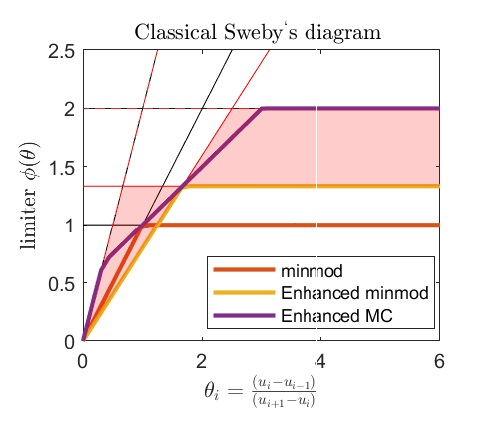
\includegraphics{limiters_original_sweby.eps}~
    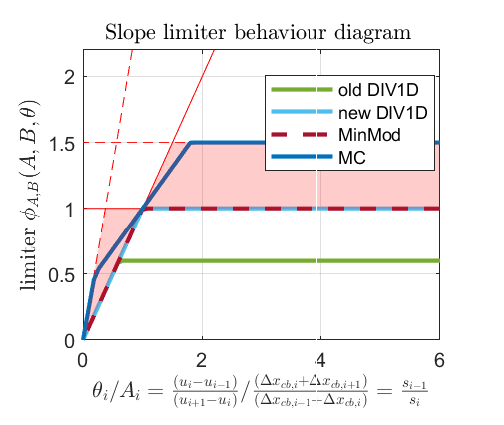
\includegraphics{limiters_adapted_sweby.eps}
    \caption{(Left) Sweby diagram and (Right) adapted Sweby diagram to show a limiter acting on slopes instead of differences.  Below the dashed lines given by Eq. \ref{eq:TVD_stable} there is TVD stability and inside the red area the limiter scheme does not loose order in the solution moving from equidistant to non-equidistant grids. On display are the MinMod , enhanced MinMod, and enhanced MC limiters for non-equidistant grid with $A=1.6,B=1.3$. The old and new DIV1D limiter schemes are also displayed on the right as function of slope.}
    \label{fig:limiters}
\end{figure}
 Using the slope limiter, the advected quantities $f$ are extrapolated to left (L) and right (R) boundary as follows:
 \begin{equation}
  f_{i}^{L,R} =   f_{i} \pm \sigma_i \cdot \Delta x_{b,i}
 \end{equation}
 Finally, the fluxes $F_{i+\frac{1}{2}} =  F_{cb,i}$ are calculated as:
 \begin{eqnarray}
     F_{cb,i} =& \frac{v_{cb,i}}{2} \left(f_{i}^{R} + f_{i+1}^{L} \right) + \underbrace{\frac{c_{s,cb,i}}{2} \left(f_{i}^{R} - f_{i+1}^{L} \right)}_{Lax ~flux} \\
      F_{cb,i} =& v_{cb,i}f_{i}^{R}\quad \quad \hbox{for $v_{cb,i}> c_{s,cb,i}$}\\
      F_{cb,i} =& v_{cb,i}f_{i+1}^{L}\quad \quad \hbox{for $v_{cb,i}< -c_{s,cb,i}$}
 \end{eqnarray}

where in addition to the slope limiter, a flux limiter is applied in the form of:
\begin{equation}
F_{i+\frac{1}{2}}=F_{i+1 / 2}^L+\varphi_{i+1 / 2}\left(F_{i+1 / 2}^H-F_{i+1 / 2}^L\right)
\end{equation}
which switches between zero and one if the velocity at the boundary exceeds the speed of sound (i.e. $|v_{cb,i}| > c_{s,cb,i} $) switching to a first order upwind or downwind scheme depending on the sign of the supersonic velocity.
For the subsonic flow, the higher order central scheme is used where the Lax flux is added to damp discontinuities allowed in the solution by the slope limiters. Note thus that there is two types of limiters, a slope limiter $\phi_{i}$ different for each cell due to the non-equidistant grid and flux limiter $\varphi$ switching integration methods. Pressure gradients are discretized using a centered scheme for non-equidistant grids. For more details see Dudson et al. and Zeng et al. \cite{dudson2019,zeng2013} and references therein.
     
For the full equations this entails the following schematics for the density, momentum, and energy equations with $i$ denoting the cell with upper and lower cell boundaries + and - respectively:
\begin{eqnarray}
    \dot{Y}_{i} \equiv& - B_i \left( \Gamma_{n/B,i}^+ -\Gamma_{n/B,i}^- \right)/ \Delta x_{\rm cb,i} + S_{n,i} &\quad\quad\hbox{for $i = 1 \cdots N$}, \nonumber \\ \nonumber \\
    \dot{Y}_{N + i} \equiv& \frac{\partial n_{\rm i}mv_{\rm i}}{\partial t} = -  B_i \left( \Gamma_{nmv/B,i}^+ -\Gamma_{nmv/B,i}^- \right)/\Delta x_{\rm cb,i} - \frac{(p_i-p_{i-1})}{2\Delta x_{i-1}} - \frac{(p_{i+1}-p_{i})}{2\Delta x_{i}} + S_{{\rm mom},i},&\quad\quad\hbox{for $i = 2 \cdots N-1$}, \nonumber \\ \nonumber \\
    \dot{Y}_{2N + i} \equiv& \frac{\partial 3n_{\rm i}eT}{\partial t} = -  B_i \left( \Gamma_{q/B,i}^+ -\Gamma_{q/B,i}^- \right)/\Delta x_{\rm cb,i} + \frac{v_{\|,i}(p_i-p_{i-1})}{2\Delta x_{i-1}} + \frac{v_{\|,i}(p_{i+1}-p_{i})}{2\Delta x_{i}} + S_{{\rm ene},i},&\quad\quad\hbox{for $i = 2 \cdots N-1$}, \nonumber \\ \nonumber \\
     \dot{Y}_{3N + i} \equiv& -\frac{\partial n_{n,i}}{\partial t} =-\left( \Gamma_{ ato,i}^+ -\Gamma_{ato,i}^- \right)/\Delta x_{\rm cb,i} + S_{{\rm neutral},i},&\quad\quad\hbox{for $i = 2 \cdots N-1$}, \nonumber \\ \nonumber \\
     \dot{Y}_{4N + i} \equiv& \frac{\partial n_{\rm ato, i}mv_{\rm ato,i}}{\partial t} = - \left( \Gamma_{n_{\rm ato}mv_{\rm ato,i}}^+ -\Gamma_{n_{\rm ato}mv,i}^- \right)/\Delta x_{\rm cb,i} + S_{{\rm ato,mom},i},&\quad\quad\hbox{for $i = 2 \cdots N-1$}, \nonumber \\ \nonumber \\
      \dot{Y}_{5N + i} \equiv& -\frac{\partial n_{m,i}}{\partial t} =-\left( \Gamma_{ mol,i}^+ -\Gamma_{mol,i}^- \right)/\Delta x_{\rm cb,i} + S_{{\rm molecule},i},&\quad\quad\hbox{for $i = 2 \cdots N-1$}, \nonumber \\ \nonumber \\
\end{eqnarray}
At the boundaries the central the pressure gradients are calculated by forward or backward differences whereas the fluxes on target boundaries are determined by the boundary conditions.  The fluxes of atoms and molecules on the cell boundaries are calculated by differences on the diffusion and for the advected atom flux using the slope limiter.
\newpage 
\subsection{Boundary conditions}

\subsubsection{X-point BC}
When simulating from the X-point to the target it is not trivial to set the upstream boundary conditions. When DIV1D uses 100\% target recycling and no cross-channel neutral losses or sources, the initial conditions will determine the outcome. For instance, the initial velocity and plasma density will determine the number of particles that can be distributed over the scrape-off layer. 
The upstream boundary condition for the ion density is set by a Dirichlet boundary condition where a time-derivative is set to evolve for time as follows. 
\begin{eqnarray}
     \dot{Y}_{\rm 1} & \equiv {\tt density\_ramp\_rate}  &
\end{eqnarray}
The momentum equation is solved on the X-point boundary:
\begin{equation}
   \dot{Y}_{\rm N+1} = \frac{\partial n_{\rm 1}mv_{\rm 1}}{\partial t} = - \left( \Gamma_{nmv/B,1}^+ -\Gamma_{nmv/B,1}^- \right)/\Delta x_{\rm cb,1} - (p_{\rm 2}-p_{\rm 1})/\Delta x_{\rm 1} + S_{\rm mom,1},
\end{equation}
where the superscripts - and + denote the left and right boundary of the first cell. The pressure gradient is evaluated/extrapolated using a forward difference. The velocity $v^{\rm -}_{\rm 1}$ of particles that flow into the first cell is obtained with the particle balance in the first cell:
\begin{eqnarray*}
\dot{Y}_1  &= \frac{n_{\rm 1}^{\rm -} v_{\rm 1}^{\rm -}A}{V} - \frac{n_{\rm 1}^{\rm +} v_{\rm 1}^{\rm +} A}{V} +   S_{n{\rm ,1}}, \\
    n_{\rm 1}^{\rm -} &= (n_{\rm 0} + n_{\rm 1})/2 ,\\
    n_{\rm 1}^{\rm +} &= n_{\rm 1} + \frac{\Delta x_{cb,1}}{2}(n_{\rm 2}-n_{\rm 1})/( x_{\rm 2} - x_{\rm 1}),\\
    v_{\rm 1}^{\rm -} &= (v_{\rm 0} + v_{\rm 1})/2,\\
    v_{\rm 1}^{\rm +} &= v_{\rm 1} + \frac{\Delta x_{\rm cb,1}}{2}(v_{\rm 2}-v_{\rm 1})/( x_{\rm 2} - x_{\rm 1}),
\end{eqnarray*}
Assuming constant ion density above the X-point (i.e. $n_{\rm 0} = n_{\rm 1}$) and solving for $v_{\rm 0}$ one obtains:
\begin{equation}
    v_{\rm 0} = \frac{2\Delta x_{\rm cb,1}}{n_{\rm 1}}\left(\dot{Y}_1 - S_{n{\rm,1}} + n_{\rm 1} + \frac{\Delta x_{\rm cb,1}}{\Delta x_{\rm cb,1}} \frac{n_{\rm 2} -n_{\rm 1}}{2\Delta x_{\rm 1}} \right).
\end{equation}
where the source of particles in the first cell $S_{n,1}$ is governed by $\dot{Y}_{\rm 1}$.
In summary, the upstream boundary condition on the momentum equation assumes zero gradient in the density and extrapolates the pressure. With constant density this translates into an extrapolated temperature.

\subsubsection{Sheath BC}
At the target(s), the fluxes are calculated using the Bohm condition $v_{target} \geq c_{s,target}$ with $c = \sqrt{\frac{2kT}{m}}$, i.e. $v_{Bohm}=\max(|v_{target}|, c_{s,target}) \text{sign}(v_{target})$. The target velocity and temperature are extrapolated from previous cell centers using Eq. \ref{eq:cc2cb}. 
Accordingly, fluxes at the target(s) are:
\begin{eqnarray}
    \Gamma_{n,t} =& v_{Bohm}\cdot n_{t}/B_{t} \\
    \Gamma_{mom,t} =& v_{Bohm}\cdot n_{t}m v_{Bohm} / B_{t} \\
    q_{t} =& \text{sign}(v_{t})c_{s,t}\cdot \gamma n_{t} e T_{t} / B_{t} \\
      \Gamma_{ato,t} =& -(1-{\tt mol\_rec}) \Gamma_{n,t}\\
    \Gamma_{ato,mom,t} =& - \Gamma_{ato,t} \cdot \sqrt{\frac{2 \mathrm{e}T_{\rm e,t} \cdot {\tt atom\_recycle\_energy\_fraction} }{m}} 
\end{eqnarray}
In terms of equations we evaluate the following at the boundary:
\begin{eqnarray}
    \dot{Y}_{N} \equiv& - B_N \left( \Gamma_{n,t} -\Gamma_{n/B,N}^- \right)/ \Delta x_{\rm cb,2N} + S_{n,N}, & \nonumber \\ \nonumber \\
    \dot{Y}_{2N} \equiv&  = -  B_N \left( \Gamma_{mom,t} -\Gamma_{nmv/B,N}^- \right)/\Delta x_{\rm cb,N} - \frac{(p_N-p_{N-1})}{\Delta x_{N-1}} + S_{{\rm mom},N},& \nonumber \\ \nonumber \\
    \dot{Y}_{3N} \equiv& = -  B_N \left( q_t -\Gamma_{q/B,N}^- \right)/\Delta x_{\rm cb,N} + \frac{v_{\|,N}(p_N-p_{N-1})}{\Delta x_{N-1}} + S_{{\rm ene},N},& \nonumber \\ \nonumber \\
     \dot{Y}_{4N} \equiv& -\left( \Gamma_{ato,t} - D(n_{cb,N-1},T_{cb,N-1})\frac{n_{n,N}-n_{n,N-1}}{\Delta x_{N-1}} \right)/\Delta x_{\rm cb,N} + S_{{\rm neutral},N},&\quad \nonumber \\ \nonumber \\
      \dot{Y}_{5N} \equiv&  = - \left( \Gamma_{ato,mom,t} -\Gamma_{atomv,N}^- \right)/\Delta x_{\rm cb,N}  + S_{{\rm ato mom},N},& \nonumber \\ \nonumber \\
      \dot{Y}_{6N} \equiv& -\left( \Gamma_{mol,t} - D_m(n_{cb,N-1},T_{cb,N-1})\frac{n_{m,N}-n_{m,N-1}}{\Delta x_{N-1}} \right)/\Delta x_{\rm cb,N} + S_{{\rm molecule},N},&\quad \nonumber \\ \nonumber \\
\end{eqnarray}
These boundaries are mirrored on the first cells if simulating with two targets.

\subsubsection{Stagnation point}
For simulations starting at the core stagnation point, the fluxes at the stagnation point are simply set to zero enforcing zero gradient in all solutions. 

\subsection{Geometry leakage for neutrals}
The neutrals do not experience the magnetic field. This means that whereas the plasma volumes are tapered to mimic flux expansion, the neutral fluxes in the SOL are calculated as if the volumes are all equal. This is inconsistent with the plasma volumes that are used and therefore a correction is applied. We denote two cells: 1 and 2 with volumes $V_{ \mathrm{1,2}}$ and widths $\Delta x_{ \mathrm{cb,1,2}}$. The flux of neutrals between the cells is determined by solving the corresponding PDE, is defined on the cell boundary. For the plasma the area of this boundary is the same for cells 1 and 2, but for the neutrals the area's differ. Namely cell 1 and two have areas $A_{1,2}= V_{ \mathrm{1,2}}/\Delta x_{ \mathrm{cb,1,2}}$ 
So, for a given flux through the boundary between the cells, directed from 1 to 2, $\Gamma_{\mathrm{cb}} ~ \mathrm{[\# m^{-2} s^{-1}]}$. The source resulting from this flux in both cells equals

\begin{align}
    S_\mathrm{1} = -\Gamma_{\mathrm{cb}}\cdot A_1 \\ 
    S_\mathrm{2} = \Gamma_{\mathrm{cb}} \cdot A_2 
\end{align}
So the difference they see is due to an apparent difference in area of the cells. However, there are a few considerations to make in dealing with this inconsistency
\begin{enumerate}
    \item if a flux goes from small to large cell, no more particle than leave the small cells may enter the large one.
    \item if a flux goes from a large cell to a small one, a part of the flux is lost.
\end{enumerate}
this results in the following four options:
\begin{equation}
\begin{aligned}
       S_{conf} = A_2\cdot \Gamma_{\mathrm{cb}}, \quad  S_{leak} = (A_1-A_2)\cdot \Gamma_{\mathrm{cb}}   \quad \for \Gamma_{\mathrm{cb}} > 0  \and A_{1} > A_2\\
       S_{conf} = A_2\cdot \Gamma_{\mathrm{cb}}, \quad  S_{leak} = 0 \quad \for \Gamma_{\mathrm{cb}} < 0  \and A_{1} > A_2\\
           S_{conf} = A_2\cdot \Gamma_{\mathrm{cb}}, \quad  S_{leak} = (A_2-A_1)\cdot \Gamma_{\mathrm{cb}}   \quad \for \Gamma_{\mathrm{cb}} > 0  \and A_{1} <  A_2\\
               S_{conf} = A_1\cdot \Gamma_{\mathrm{cb}}, \quad  S_{leak} =0  \quad \for \Gamma_{\mathrm{cb}} < 0  \and A_{1} < A_2,
\end{aligned}
\end{equation}
where the confined and leaking sources are calculated. These are included in the terms describing flows between external reservoirs and SOL.


% At the target(s), all momentum sources are neglected and the static pressure is assumed to be constant. The target boundary for momentum is then solved through backward differences and linear extrapolation of the ion density and temperature in a mirrored target as follows:
% \begin{equation}
%    \dot{Y}_{\rm 2N} = \frac{\partial n_{\rm N}mv_{\rm N}}{\partial t} = - \left(n_{\rm N} m v_{\rm N}^2 - n_{\rm N-1} m v_{\rm N-1}^2 \right)/\Delta x_{\rm N} - (p_{\rm N}-p_{\rm N-1})/\Delta x_{\rm N-1} 
% \end{equation}
% (CHECK THIS)

\section{Input and Output}\label{IO}

Here we provide a complete list of the input and output parameters of the code. The input is read from a file named {\tt input.txt} in the directory in which the code is executed. The input is read in the form of two FORTRAN namelists. The first namelist contains the settings of the numerical parameters for the code as listed in table~\ref{tab:input_numerics}. The second namelist contains the settings for the physics parameters as listed in table~~\ref{tab:input_physics}. Some inputs can be switched to be dynamic, which requires additional files in the execution director. These files should only contain columns with numerical values and indicated sizes. \\

The output is written in the execution directory in {\tt div1doutput.txt}. Firstly, most inputs that were provided via {\tt input.txt} and the {\tt *.dat} files have been appended to {\tt div1doutput.txt} in the Fortran namelist format and represent the actual values used by DIV1D for input verification. This includes the geometry. Secondly, the outputs in terms of states: {\tt density, velocity, temperature, neutral, neutral momentum, molecules }, fluxes: {\tt Gamma\_n, Gamma\_mom, q\_parallel, neutral\_flux, neutral\_momentum\_flux, molecule\_flux }, and sources: {\tt Source\_n, Source\_v, Source\_Q, Source\_neutral, Source\_neutral\_mom, Source\_molecule} are written. The outputs of the external reservoir and core are written in a similar fashion. The flows of particles going from one domain to another are written twice, once for each domain and listed as, e.g. {\tt sol2extern\_flux(5), extern2sol\_flux(Nx), sol2core\_flux(1), core2sol\_flux(Nx), core2extern\_flux(5), extern2core\_flux(1) }, this way conservation of quantities between domains can be verified. Similarly molecule flows are written to variables where {\tt flux} is replace by { \tt mol }. 

% \begin{table}[h]
% \begin{center}
\begin{longtable}{| p{.25\textwidth} | p{.78\textwidth} |} 
  \caption{{\bf Namelist {\tt div1d\_numerics} setting parameters controlling the numerical implementation}.}  
  \label{tab:input_numerics} 
  \hline 
        variable name                & description \\ \hline \hline
    {\tt Nx}                     & integer: number of points in the grid along the field line (default: 1000) \\ \hline
    {\tt ntime}                  & integer: number of times steps (default: 1000)  \\ \hline
    {\tt delta\_t}               & real: time step size (default: 1.0D-06)  \\ \hline
    {\tt nout}                   & integer: output is written to file every time steps (default: 100) \\ \hline
    {\tt nout\_steps}                   & integer: number of times nout steps are taken (default: 10) \\ \hline
    {\tt method}                 & integer: set method flag for {\tt dvode} integrator (default: 227)   \\ \hline
	{\tt istate\_mod}            & integer: number of time steps between calls to {\tt dvode} with {\tt istate = 1} (default: 0) \\ \hline
	{\tt max\_step}              & integer: maximum number of internal steps in {\tt dvode} (default: 100000) \\ \hline
	{\tt max\_attempts}          & integer: maximum number of restarts of {\tt dvode} after failed integration (default: 1000) \\ \hline
    {\tt abstol}                 & real: absolute value of tolerance in numerical integration (default: 1.0D-4)  \\ \hline
    {\tt reltol}                 & real: relative value of tolerance in numerical integration (default: 1.0D-4)  \\ \hline
	{\tt evolve\_density}        & integer: multiplier for density evolution (default: 1) \\ \hline
	{\tt evolve\_momentum}       & integer: multiplier for momentum evolution (default: 1) \\ \hline
	{\tt evolve\_energy}         & integer: multiplier for energy evolution (default: 1) \\ \hline
	{\tt evolve\_neutral}        & integer: multiplier for neutral density evolution (default: 1) \\ \hline
    {\tt evolve\_neutral\_momentum} & integer: multiplier for neutral momentum density evolution (default: 1) \\ \hline
    {\tt evolve\_molecule}        & integer: multiplier for molecule density evolution (default: 1) \\ \hline
    {\tt evolve\_background(5)}        & integer: multiplier for neutral density evolution (default: (0, 0, 0, 0, 0)) \\ \hline
    {\tt evolve\_core}        & integer: multiplier for evolving the core density (default: 0) \\ \hline
	{\tt density\_norm}          & real: normalization of densities in solution vector {\tt Y} (default: {\tt initial\_n}) \\ \hline
	{\tt temperature\_norm}      & real: temperature used to normalize solution vector {\tt Y} (default: 1.0D0 eV) \\ \hline
	{\tt velocity\_norm}         & real: velocity used to normalize solution vector {\tt Y} (default: sound speed at {\tt temperature\_norm}) \\ \hline
	{\tt switch\_density\_source} & real: multiplier of source term in particle balance (default: 1.0D0) \\ \hline
	{\tt switch\_momentum\_source}& real: multiplier of source term in momentum balance (default: 1.0D0) \\ \hline
	{\tt switch\_energy\_source}  & real: multiplier of source term in energy balance (default: 1.0D0) \\ \hline
	{\tt switch\_neutral\_source} & real: multiplier of source term in neutral density equation (default: 1.0D0) \\ \hline
	{\tt switch\_charge\_exchange}& real: multiplier of the charge exchange rate (default: 1.0D0) \\ \hline
	{\tt switch\_recombination}  & real: multiplier of the recombination rate (default: 1.0D0) \\ \hline
	{\tt switch\_ionization}     & real: multiplier of the ionization rate (default: 1.0D0) \\ \hline
	{\tt switch\_excitation}     & real: multiplier of the excitation rate (default: 1.0D0) \\ \hline
	{\tt switch\_impurity\_radiation}& real: multiplier of the impurity radiation losses (default: 1.0) \\ \hline
	{\tt viscosity}              & real: numerical viscosity (default: 0.0D0)  \\ \hline
	%{\tt central\_differencing}   & real: fraction of central differencing in pressure gradient term (default: 0.5D0) \\ \hline
    {\tt lax\_switch}        & real: multiplier for lax-flux in advection routine (default: 1) \\ \hline
	{\tt restart}                & logical: when {\tt .true.} initial conditions are read from restart file (default: {\tt .false.}) \\ \hline
    \hline
\end{longtable}
% \begin{table}[h]
% \begin{center}
  
  % 
%  \begin{tabular}{|| l  | l ||}
  % \begin{tabular}{@{}|l|l| }
  \FloatBarrier
\newpage
    \begin{longtable}{| p{.25\textwidth} | p{.78\textwidth} |} 
    \caption{{\bf Namelist {\tt div1d\_physics} setting parameters controlling the physics implementation}.}
    \hline
    {variable name }              & description \\ \hline \hline 
    {\tt L}                       & real: length of the field line between X-point and target (default: 5.0D1~m) \\ \hline
    {\tt L\_core\_SOL}            & real: length of the field line between X-points(default: 0.0D0~m) \\ \hline
    {\tt X\_core\_SOL}            & real: first X-point position (default: 0.0D0~m) \\ \hline
    {\tt L\_baffle}               & real: Length along flux tube from X-point to baffle: (default: 0.0D0~m) \\ \hline
    {\tt mass}                    & real: mass of the main plasma ion (default: 3.3436D-17~kg for D) \\ \hline
    {\tt gamma}                   & real: sheath heat transmission factor (default: 6.5D0) \\ \hline
    {\tt sintheta}                & real: sinus of angle theta between B-field and target plate (default: 0.1D0)(-1 req {\tt sintheta.dat}) \\ \hline
    {\tt q\_parX}                 & real: parallel heat flux at the X-point (default: 1.0D8~W/m$^2$)  (-1 req {\tt dyn\_qpar.dat})  \\ \hline
    {\tt Gamma\_X}                & real: parallel heat flux at the X-point (default: 1.0D8~W/m$^2$) \\ \hline
    {\tt Gamma\_core}             & real:  particle flux coming from the core boundary when {\tt L\_core\_SOL} .gt. 0 (default: 1D21$ ~s^{-1}$)  (-1 req {\tt dyn\_gamma\_core.dat})  \\ \hline
    {\tt Q\_core}                 & real: heat flux coming from the core boundary when {\tt L\_core\_SOL} .gt. 0  (default: 8.0D6)  (-1 req {\tt dyn\_q\_core.dat})  \\ \hline
    {\tt alpha\_core\_profile\_n}  & real:  parameter describing the ballooning of the core particle losses (default: 1.0D0) \\ \hline
    {\tt alpha\_core\_profile\_Q}  & real:  parameter describing the ballooning of the core energy losses (default: 1.0D0) \\ \hline
    {\tt flux\_expansion}         & real: expansion of magnetic flux from X-point to target (default: 1.0D0) (-1 req {\tt B\_field.dat})\\ \hline
    {\tt trans\_expansion}        & real: expansion of transport flux from X-point to target (default: 1.0D0) (-1 req {\tt B\_trans.dat})\\ \hline
    {\tt initial\_n}              & real: initial, homogeneous particle density (default: 1.0D20~m$^{-3}$) (X-point BC with -1 req {\tt dyn\_nu.dat})) \\ \hline
    {\tt initial\_v}              & real: initial, homogeneous plasma velocity (default: 0.0D0~m/s) \\ \hline
    {\tt initial\_vn}             & real: initial, homogeneous atomic velocity (default: 0.0D0~m/s) \\ \hline
    {\tt initial\_T}              & real: initial, homogeneous plasma temperature (default: 1.0D2~eV) \\ \hline
    {\tt initial\_a}              & real: initial, homogeneous atomic density (default: 1.0D14~m$^{-3}$) \\ \hline
    {\tt initial\_m}              & real: initial, homogeneous molecule density (default: 1.0D14~m$^{-3}$) \\ \hline
    {\tt initial\_ncore}          & real: initial, core electron density (default: 1.0D14~m$^{-3}$) \\ \hline
    {\tt initial\_core\_neutral}  & real: initial, core atom density (default: 1.0D14~m$^{-3}$for connection to core neutral model) \\ \hline
    {\tt initial\_nb(5)}          & real: initial, atomic density in reservoirs (default: 1.0D17~m$^{-3}$) (-1 req {\tt dyn\_nb.dat}) \\ \hline
    {\tt initial\_mb(5)}         & real: initial, molecule density in reservoirs (default: 1.0D17~m$^{-3}$)  (-1 req {\tt dyn\_mb.dat})  \\ \hline
     {\tt density\_ramp\_rate}    & real: rate of change of X-point density (default: 0.0D0~/m$^3$/s) \\ \hline
    {\tt impurity\_concentration(1:5)} & real: concentration of impurity ions (default: 1.0D-2) (-1 req {\tt dyn\_imp\_con.dat}) \\ \hline
    {\tt impurity\_Z(1:5)}      & Integer: mass of the impurity ion (default: 6) \\ \hline
    {\tt switch\_impurity\_dist}& switch to load in impurity profiles from {\tt prf\_imp\_dis.dat} (default = homogeneous) \\ \hline
    {\tt core\_ionization\_frac } & real: fraction of the neutrals that passes the sol and ionizes in the core (default: 0.0D0) \\ \hline
       {\tt core\_ion\_frac\_mol } & real: fraction of the molecules that passes the sol and ionizes in the core (default: 0.0D0) \\ \hline 
    {\tt  pol\_target\_angle(2)}& real: poloidal angle at target 1,2 (default: [90d+0,90d+0]) \\ \hline  
    {\tt sol\_width\_omp}       & real: width of the core SOL at the outer midplane (default: 3.0d-2 m)\\ \hline  
    {\tt location\_omp }        & real: relative position of the outer midplane on the core SOL [0,1] 	(default: 0.5d+0) \\ \hline 
    {\tt major\_radius }        &  real:  major radius of the core SOL [m] (default: 0.9d+0) (-1 requires {\tt major\_radius.dat})\\ \hline    
    - & DIV1D will look for additional geometric SOL information {\tt major\_height.dat} and  {\tt sol\_normal.dat} pointing to the core having Nx entries. \\ \hline 
    - & DIV1D will look for vessel information   {\tt vessel\_r.dat}, {\tt vessel\_z.dat} having Nv $>$ 9 entries, holding the radial and vertical position array of a wall going from the surface in PFR reservoir 1 clock-wise through 2 DFR, 3 CFR , 4 DFR, to PFR reservoir 5. \\
    - & DIV1D will look for  {\tt vessel\_c.dat} (size Nv) with zeros (false) and precisely 9 entries of unity (true) marking connection points to reservoirs with (1) intersection PFR r5-1, (2) strike-point PFR r1, (3) strike-point DFR r2, (4) baffle-point r2-3, (5) stagnation point CFR r3, (6) baffle-point r3-4, (7) strike-point DFR r4, (8) strike-point PFR r5, (9) intersection PFR r5-1. \\ \hline
    {\tt recycling}             & real: fraction of ion flux on target recycled as neutral (default: 1.0D0) \\ \hline
    {\tt atom\_recycle\_energy\_fraction} & real: fraction of ion target energy returned in recycled atoms (default: 0.2) \\ \hline
    {\tt mol\_rec}              & real: fraction of target ions recycling into molecules (default: 0.0) \\ \hline
    {\tt wall\_association\_prob} & real: probability of atoms incident on reservoir wall to associate (default: 0.0) \\ \hline
    {\tt neutral\_residence\_time}   & real: inverse exchange velocity for atoms between sol and reservoirs (default: 1.0D20~s/m) \\ \hline
    {\tt molecule\_residence\_time}  & real:  inverse exchange velocity for molecules between sol and reservoirs (default: 1.0D20~s/m) \\ \hline
    {\tt ato\_res\_asy}          & real: asymmetric atom exchange for difference in SOL/reservoir temperature (default: 1) \\ \hline
    {\tt mol\_res\_asy}          & real: asymmetric molecule exchange for difference in SOL/reservoir temperature (default: 1) \\ \hline 
    {\tt gas\_puff\_source}      & real: total particle source from gass puff along flux tube (default: 0.0D0~m$^{-2}$) \\ \hline
    {\tt gas\_puff\_location}    & real: location of gas puff along flux tube (default: 0.0D0~m) \\ \hline
    {\tt gas\_puff\_width}       & real: Gaussian width of gas puff region along flux tube (default: 1.0D20~m) \\ \hline
    {\tt charge\_exchange\_model}& character string selecting the charge exchange model (default: {\tt AMJUEL}) \\ \hline
    {\tt ionization\_model}      & character string selecting the ionization model (default: {\tt AMJUEL}) \\ \hline
    {\tt recombination\_model}   & character string selecting the recombination model (default: {\tt AMJUEL}) \\ \hline
    {\tt energy\_loss\_ion}      & real: effective energy loss per ionization (only used when {\tt switch\_excitation .eq. 0.0d+0})) \\ \hline
    {\tt neutral\_energy}        & real: average energy of neutrals [eV] (default: 5~eV) ($-Y$ function of plasma $T$: $E= Y\cdot T$)\\ \hline
    {\tt minimum\_density}       & real: minimum value allowed for densities (default: 1.0D4~m$^{-3}$) \\ \hline
    {\tt minimum\_temperature}   & real: minimum value allowed for temperatures (default: 0.1D0~eV) \\ \hline
    {\tt elm\_start\_time}   	 & integer: outer time step at which the first ELM starts, in units of delta\_t (default: 0) \\ \hline
    {\tt elm\_ramp\_time}   	 & integer: ramp time of ELM (not exact for gaussian, see section~\ref{section:elms}), in units of delta\_t (default: 0) \\ \hline
    {\tt elm\_time\_between}     & integer: outer time steps between two the start of two ELMs, in units of delta\_t (default: 2d+08) \\ \hline
    {\tt elm\_expelled\_heat}    & real: total amount of expelled heat per unit area due to an ELM (default: 0 J m$^{-2}$) \\ \hline
    {\tt elm\_expelled\_particles}& real: total number of expelled particles due to an ELM (default: 0 m$^{-3}$) \\ \hline
    {\tt switch\_elm\_heat\_flux}& integer: turns off (0) or on (1) the ELM contribution to the heat flux (default: 0) \\ \hline
    {\tt switch\_elm\_density}   & integer: turns off (0) or on (1) the ELM contribution to the particle flux (default: 0) \\ \hline
    {\tt switch\_elm\_series}    & integer: turns off (0) or on (1) the multi-ELM sequence (default: 0) \\ \hline
    {\tt gaussian\_elm}          & integer: chooses triangular (0) or gaussian (1) ELM (default: 0) \\ \hline
    {\tt extern\_neutral\_volumes }   & real: volumes of external reservoirs (default: [0.6d0,0.1d0,5.0d+0,1.2d0,0.6d0]~m3)\\ \hline 
    {\tt extern\_neutral\_wall\_area(5)} & real: (1) inner PFR, (2) inner divertor CFR, (3) CFR, (4) outer divertor CFR, (5) outer PFR \\ \hline
    {\tt  extern\_neutral\_ex(3) }    & real: clockwise external atom flows (1) = (5$\rightarrow$1),(2) = (2$\rightarrow$3),(3) =(3$\rightarrow$4) (default: 0)  [1/s]  \\ \hline
    {\tt extern\_molecule\_ex(3)} & real: clockwise external molecule flows: (1) = (5$\rightarrow$1),(2) = (2$\rightarrow$3),(3) =(3$\rightarrow$4)  (default: 0)  [1/s]    \\ \hline
    {\tt  pol\_target\_parallel\_angle(2)} & real: poloidal angle at target 1,2 (between 0-180) [deg]  \\ \hline 
    {-} & for 0 fluxes $\rightarrow$ 1 and 4, for 180 all flux $\rightarrow$ 2 and 5. (default:  (90d+0,90d+0)) [deg] \\ \hline
    {\tt  puff\_rate\_neutral(5) } & real: puff rate of neutral atoms in background chamber (default: 0) [D/s] (-1 req {\tt neutral\_puff.dat}) \\ \hline
    {\tt puff\_rate\_molecule(5) }      & real: puff rate of neutral molecules in background chamber (default:0) [D2/s] (-1 req {\tt molecule\_puff.dat}) \\ \hline
    {\tt  pump\_rate\_n(5) }            & real: pump rate of atoms in background chamber  (default: 0 ) [1/s]\\ \hline
    {\tt  pump\_rate\_m(5) }            & real:  pump rate of molecules in background chamber  (default: 1 ) [1/s]\\ \hline
    {\tt   core\_confinement\_time  }   & real: confinement time of particles in the core (default: 0.2 ) [s]\\ \hline    
    {\tt  core\_fuelling	}           &  real: core fuelling rate, e.g. pellet injection or NBI (default: 1.0d+22)  [1/s] (-1 req {\tt dyn\_core\_fuelling.dat}) \\ \hline 
    {\tt  core\_volume }                & real: volume of core plasma (default: 5) [m$^3$] \\ \hline 
    {\tt core\_ext\_neutral\_pump(5)  } & real: The core, pumping external atoms directly (default: 0 ) [1/s]\\ \hline
    {\tt core\_ext\_molecule\_pump(5) } & real: The core, pumping external molecules directly  (default: 0) [1/s]\\ \hline
    {\tt core\_far\_sol\_ion\_loss  }   & real: loss of ions to the far scrape-off layer in the core-sol   (default: 0 ) [-]\\ \hline 
    {\tt  core\_far\_sol\_feedthrough } & real: direct feed-through of core flux to the main chamber (not tested!) [-]) \\ \hline 
    {\tt core\_ionization\_fraction }   & real: fraction of atoms from external reservoir that ionize in the core (default: 0 ) [-]\\ \hline
    {\tt core\_ionization\_fraction\_mol} & real: fraction of molecules from external reservoir that ionize in the core (default: 0 ) [-]\\ \hline    
    {\tt core\_sol\_neutral\_ex}        & real: core neutral ex between sol and core [m/s] (for connection to core model)   \\ \hline  
    {\tt  sigma\_nb  }                  &  real: spread of sigmoid function for reservoir densities near. (default: 1D-10) [-]   \\ \hline    
    \end{longtable}
\cleardoublepage
\section{Tests} 
In addition to being version controlled, there are some tests implemented to keep the model environment healthy.\\
\begin{itemize}
    \item \textbf{Integration tests:}There is a set of tests available with standard inputs to investigate if new features do not break configurations in which they are not developed.
    \item \textbf{Regression tests:} There is a set of regression tests available (through the Matlab wrapper) that in parallel run different configurations to a stationary solutions and in post-processing (using output of DIV1D) evaluate if the equations as listed in this manual are satisfied to numerical accuracy of the written solutions.
    \item \textbf{Unit tests:} an effort is made to have routines that are unit-testable in order to test parts of the code specifically for particle conservation.
\end{itemize}
\\

\section{DIV1D as a library}
\noindent There is the option to compile DIV1D as a shared-object file. This stand-alone library offers communication through memory and therefore integration in larger code-suites. As of January 2025, interfaces to Matlab, C and Python are supported. A combined Musscle3.0 and IMAS interface is under development. \\

\noindent In addition to an interface alone, the library offers tight control over the particle flows over the seperatrix during time-integration. Specifically these flows can be frozen over a number of time-integration steps. In a Gauss Seidel style solver of coupled systems of equations this can be used to ensure particle conservation in a single forward Euler time integration step. Removing the need for subsequent calls to DIV1D for convergence in the solutions. This will help DIV1D not too slow-down a much faster core-solver.\\

\noindent For speed, the numerical settings of DIV1D can be loosened, a minimum time-step can be set, but no implicit time-step solver is tested in the present version. This means that as soon as the dynamics become interesting, fast, chaotic, dynamic, etc.. the solver will reduce its time-step to converge and slow down. Still, obtaining a stationary solution for the SOL requires roughly a minute on an intel Xeon CPU from 2011 and simulation a second of global plasma should finish in 1 to 12 hours. This really depends on how challenging the scenario is, the 12 hour case is for a simulation running a multisine perturbation between 1 and 600 Hz, writing solutions every 10 microseconds, while it takes roughly 1 hour on TCV to simulate flat-top. For reliable real-time needs, it is advised to generate a data-set (this can be done overnight) and refer to standard and or neural based acceleration techniques. See e.g. \cite{poels2023}\\



\cleardoublepage
\section{Benchmark with 2 Point Model}
The 2 Point Model for an attached divertor plasma assuming purely conductive heat transport and no losses is discussed in Chapter 5.2 of~\cite{stangeby}). For a given parallel heat flux $q_{\parallel,\rm X}$ entering the divertor leg upstream, a given upstream plasma density $n_{\rm X}$, the length of the divertor leg $L$, and neglecting possible effects of flux expansion a set of three equations is obtained from the energy balance, the sheath heat transmission, and pressure balance respectively~\cite{stangeby}:
\begin{equation}\label{2PM_energy_balance}
    T_{\rm X} = \left(T_{\rm L}^{7/2} + {7 \over 2} {q_{\parallel,\rm X} L \over \kappa_0}\right)^{2/7},
\end{equation}
\begin{equation}\label{2PM_sheath_heat_transmission}
    q_{\parallel,\rm X} = \gamma n_{\rm L} e T_{\rm L} c_{\rm s},
\end{equation}
\begin{equation}\label{2PM_pressure_balance}
    2 n_{\rm L} T_{\rm L} = n_{\rm X} T_{\rm X}.
\end{equation}
with $\kappa_0 = 2000$~W/eV$^{7/2}$m. These equations can be used to solve for the three unknowns, upstream temperature $T_{\rm X}$, target temperature $T_{\rm L}$ and target density $n_{\rm L}$. The solution can be obtained iteratively starting from $T_{\rm L} = 0$. In the first iteration the solution for $T_{\rm X}$ then is
\begin{equation}\label{2PM_upstream_temperature}
    T_{\rm X} = \left({7 \over 2} {q_{\parallel,\rm X} L \over \kappa_0}\right)^{2/7}.
\end{equation}
Next an equation for $T_{\rm L}$ is obtained by substituting equation (\ref{2PM_pressure_balance}) in the sheath heat transmission (\ref{2PM_sheath_heat_transmission}):
\begin{equation}\label{2PM_target_temperature}
    T_{\rm L} = {m \over e} {2 q_{\parallel,\rm X}^2 \over \gamma^2 e^2 n_{\rm X}^2 T_{\rm X}^2}.
\end{equation}
Finally the pressure balance (\ref{2PM_pressure_balance}) then allows to obtain the target density as
\begin{equation}\label{2PM_target_density}
    n_{\rm L} = {\gamma^2 e^3 n_{\rm X}^3 T_{\rm X}^3 \over 4 m q_{\parallel,\rm X}^2}.
\end{equation}
In fact, these last three equations represent the simple 2 Point Model as obtained under the condition that $T_{\rm X} \gg T_{\rm L}$ \cite{stangeby}.

An extension of the simple 2 Point Model is obtained introducing the effects of a finite convective contribution to the parallel heat transport, as well as power and momentum losses (see Chapter 5.4 of~\cite{stangeby}). Assuming that the convective contribution is evenly distributed over the distance between the X-point and target, the solution to the energy balance equation \ref{2PM_energy_balance} is simply modified as
\begin{equation}\label{extended_2PM_energy_balance}
    T_{\rm X} = \left(T_{\rm L}^{7/2} + {7 \over 2} {q_{\parallel,\rm X} (1 - f_{\rm conv}) L \over \kappa_0}\right)^{2/7},
\end{equation}
introducing the factor $f_{\rm conv}$ representing the relative contribution from convection to the heat transport. When the power and momentum losses are not negligible yet sufficiently localized near the target, the energy balance solution for the upstream temperature (\ref{extended_2PM_energy_balance}) is not altered further, while the sheath heat transmission is simply modified by introducing the factor $(1-f_{\rm pwr})$ on the left hand side of equation (\ref{2PM_sheath_heat_transmission}) and the pressure balance is modified similarly by introducing the factor $(1-f_{\rm mom})$ on the right hand side of equation (\ref{2PM_pressure_balance}) to account for the power an momentum losses, respectively. As a result the equation for the target temperature (\ref{2PMF_target temperature}) is modified to
\begin{equation}\label{extended_2PM_target_temperature}
    T_{\rm L} = {m \over e} {2 q_{\parallel,\rm X}^2 (1-f_{\rm pwr})^2 \over \gamma^2 e^2 n_{\rm X}^2 T_{\rm X}^2 (1-f_{\rm mom})^2}.
\end{equation}
while the target density is modified to
\begin{equation}\label{extended_2PM_target_density}
    n_{\rm L} = {\gamma^2 e^3 n_{\rm X}^3 T_{\rm X}^3 (1-f_{\rm mom})^3 \over 4 m q_{\parallel,\rm X}^2 (1-f_{\rm pwr})^2}.
\end{equation}
The power and momentum loss fractions $f_{\rm pwr}$ and $f_{\rm mom}$ are defined as
%\begin{equation}\label{power_loss_fraction}
%    f_{\rm pwr} \equiv \int_{x=L}^0 Q {\rm d}x \Big/ q_{\parallel,\rm X},
%\end{equation}
\begin{equation} \label{power_loss_fraction}
f_{\rm pwr} \equiv \left(1-\frac{q_{\mathrm{\|,L}} }{q_{\mathrm{\|,X}}} \frac{B_{\mathrm{X}}}{B_{\mathrm{L}}}\right)=\int_{x=L}^{0}\left[\frac{v_{\|}}{B} \frac{\partial p}{\partial x}+\frac{Q}{B}\right] d x \frac{B_{\rm X}}{q_{\mathrm{\|,X}}}
\end{equation}
and
%\begin{equation}\label{momentum_loss_fraction}
%    f_{\rm mom} \equiv \int_{x=L}^0 S_{\rm mom} {\rm d}x \Big/ p_{\rm tot,X},
%\end{equation}
\begin{equation}\label{momentum_loss_fraction}
f_{\rm mom} \equiv 1-\frac{p_{\rm tot,L}}{p_{\rm tot,X}}=\int_{x=L}^{0}\left(-n m v_{\|}^{2} \frac{\partial B}{\partial x}+S_{\rm mom}\right) d x / p_{\rm tot,X}
\end{equation}

respectively \cite{stangeby2018}. Also the equations for the extended 2 Point Model (\ref{extended_2PM_energy_balance}-\ref{extended_2PM_target_density}) are easily solved by iteration when the convective fraction, and the power and momentum loss fractions are known.

Also flux expansion can be accounted for in the 2 Point model. In case of finite flux expansion, neglecting as usual the convective transport and assuming that all sources and sinks are well localized near the target the stationary energy equation becomes
\begin{equation}
    {q_\parallel \over B} = {q_{\parallel, \rm X} \over B_{\rm X}}.
\end{equation}
The solution of this equation now results in
\begin{equation}\label{extended_2PM_energy_balance_FE}
    T_{\rm X} = \left(T_{\rm L}^{7/2} + {7 \over 2} {q_{\parallel,\rm X} (1 - f_{\rm conv}) L  \Phi_{\rm f} \over \kappa_0}\right)^{2/7},
\end{equation}
introducing the flux expansion integral $\Phi_{\rm f}$ defined as
\begin{equation}\label{FE_integral}
    \Phi_{\rm f} \equiv \int_0^1 {B\over B_{\rm X}} {\rm d}{\bar x}.
\end{equation}
Here, ${\bar x} \equiv x /L$ is the normalized $x$ coordinate. Using that $B \propto 1/R$ and assuming that the major radius varies linearly along the divertor leg this integral evaluates to
\begin{equation}\label{FE_integral_}
    \Phi_{\rm f} = \int_0^1 {1 \over 1 + \varepsilon_{\rm f} {\bar x}} {\rm d}{\bar x} = {\ln( 1 + \varepsilon_{\rm f} ) \over \varepsilon_{\rm f}},
\end{equation}
with the flux expansion parameter $\varepsilon_{\rm f}$ defined by $\varepsilon_{\rm f} \equiv (R_{\rm L}/R_{\rm X}) - 1$. A second modification to the extended 2 Point Model equations comes from the sheath boundary condition, which accounting to the flux expansion near the target is modified to
\begin{equation}\label{2PM_sheath_heat_transmission_FE}
    q_{\parallel,\rm X} {(1-f_{\rm pwr}) \over (1 + \varepsilon_{\rm f})} = \gamma n_{\rm L} e T_{\rm L} c_{\rm s}.
\end{equation}
This results in a modification of the equation for the target temperature to
\begin{equation}\label{extended_2PM_target_temperature_FE}
    T_{\rm L} = {m \over e} {2 q_{\parallel,\rm X}^2 (1-f_{\rm pwr})^2 \over (1 + \varepsilon_{\rm f})^2 \gamma^2 e^2 n_{\rm X}^2 T_{\rm X}^2 (1-f_{\rm mom})^2},
\end{equation}
and of the target density is to
\begin{equation}\label{extended_2PM_target_density_FE}
    n_{\rm L} = {\gamma^2 e^3 n_{\rm X}^3 T_{\rm X}^3 (1-f_{\rm mom})^3 (1 + \varepsilon_{\rm f})^2 \over 4 m q_{\parallel,\rm X}^2 (1-f_{\rm pwr})^2}.
\end{equation}
Again these equations (\ref{extended_2PM_energy_balance_FE}), (\ref{extended_2PM_target_temperature_FE}), and (\ref{extended_2PM_target_density_FE}) are easily solved iteratively.

For the case that the losses along the divertor leg and/or the convective heat flux are not negligible, Kotov and Reiter \cite{kotov2009} derived an exact 2 Point Model Formulation for the target temperature and density, which under the conditions of the present model (equal electron and ion temperature, sound speed at the sheath boundary, and constant magnetic field) is simplified to
\begin{equation}\label{2PMF_target temperature}
    T_{\rm L} = {8m \over e \gamma^2} {q_{\parallel,\rm X}^2 \left(1-f_{\rm pwr}\right)^2 \over p_{\rm tot,X}^2 \left(1-f_{\rm mom}\right)^2}
\end{equation}
\begin{equation}\label{2PMF_target density}
    n_{\rm L} = {\gamma^2 \over 32 m} {p_{\rm tot,X}^3 \left(1-f_{\rm mom}\right)^3 \over q_{\parallel,\rm X} \left(1-f_{\rm pwr}\right)^2}
\end{equation}
where $p_{\rm tot,X} = 2 n_{\rm X} e T_{\rm X} + n_{\rm X} m v_{\parallel\rm X}^2$ is the total upstream pressure. When the upstream parallel momentum is negligible, these equations are identical to the extended 2 Point Model equations (\ref{extended_2PM_target_temperature}) and (\ref{extended_2PM_target_density}) for the target temperature and density. These equations can serve as an accuracy check for the numerical code.


\subsection{Analytical Extended 2 Point Model}

When one would have simple closed analytical expressions for the power and momentum loss fraction, an instructive version of the extended 2 Point Model would be obtained. Such a model might provide further insight into conditions for divertor detachment and can be used for extremely fast calculations as needed in detachment control. Noting that both power losses and momentum losses typically increase with decreasing target temperature or increasing target density, we suggest the simple scaling
\begin{equation}\label{scaling_of_losses}
    f_{\rm pwr, mom} = exp( - \alpha_{\rm pwr, mom} T_{\rm L} / n_{\rm L} ),
\end{equation}
where the coefficients $\alpha_{\rm pwr, mom}$ must be chosen appropriately. Note that detachment (a decreasing target temperature) requires that $f_{\rm mom} < f_{\rm pwr}$, i.e. $\alpha_{\rm mom} < \alpha_{\rm pwr}$.

Some other remarks on the solutions of the 1D problem. Momentum dissipation requires a finite velocity, which only appears near the target where a finite particle source from ionization must be compensated by a convective particle flux towards the target. When recycling is incomplete or in case of efficient pumping in the divertor region, a significant particle flux must be present at the X-point already and there will be much more possibilities for momentum dissipation along the entire divertor leg. Impurity puffing will mostly effect power dissipation without significant momentum dissipation. In contrast, increasing the neutral density in the divertor by normal gass puff will increase the charge exchange rate and thereby increases momentum dissipation. Note that increasing the length of the divertor leg increases the X-point temperature. This must have a limit somewhere which sets a maximum distance from the X-point to the recombination front, when the divertor leg length becomes larger that this the detachment front must separate from the target. The question then arises about the stability of the detachment front position. How is this determined??


\section{Further analysis of the 1D divertor model: stationary solutions}

Important insight into the existence and stability of stationary solutions can be obtained by some further assumptions concerning the 1D model. In particular, ionization and recombination are often located in a relatively narrow zone. For stationary solutions of the equations, the pressure can then be assumed to be constant outside this narrow ionization and recombination zone and the parallel velocity and the convective heat flux can be neglected. The stationary solutions are then entirely specified by the stationary energy balance
\begin{equation}\label{stationary_energy_balance}
    {\partial \over \partial x} q_\parallel = Q \quad\hbox{with}\quad q_\parallel = - \kappa_\parallel {\partial \over \partial x} T.
\end{equation}
Using a transformation first introduced by Wim Goedheer [check citation] in the context of radiation losses from the edge of the confined plasma, allows to recast this equation into an integral equation for the change in the heat flux over the divertor leg or, in other words, an integral equation for the radiative energy losses in the divertor region. To this end Eq.~({\ref{stationary_energy_balance}) is multiplied by the parallel heat flux and integrated to obtain
\begin{equation}\label{flux_change}
    q_X^2 - q_L^2 = - 2 \int_{T_L}^{T_X} \kappa_\parallel Q {\rm d}T.
\end{equation}
Next, the parallel heat conductivity is substituted as $\kappa_\parallel = \kappa_0 T^{5/2}$, the energy loss term is taken in the form of the radiative impurity losses (\ref{impurity_radiation}), and the constant pressure, $ p = 2 neT$, approximation is applied to obtain~\cite{lengyel1981,capes1992,hutchinson1994}
\begin{equation}\label{flux_change_2}
    q_X^2 - q_L^2 = {1\over2 e^2} \kappa_0 p^2 \xi_Z \int_{T_L}^{T_X} \sqrt{T} L_Z(T) {\rm d}T,
\end{equation}
where the impurity concentration $xi_Z$ has also been assumed to be constant over the radiative layer.

A number of conclusions can be drawn from this equation. Several authors apply it to quantify the maximum flux that can be radiated away in the divertor leg \cite{lengyel1981,lackner1993,kallenbach2013,siccinio2016}
\begin{equation}\label{maximum_radiated_flux}
    q_{\rm max} = \sqrt{{1\over2 e^2} \kappa_0 p^2 \xi_Z \int_0^\infty \sqrt{T} L_Z(T) {\rm d}T}.
\end{equation}
Hutchinson and Lipschultz use it to formulate the stability condition for a radiative front~\cite{hutchinson1994,lipschultz2016}:
\begin{equation}
    {{\rm d} \over {\rm d}x_f} (q_i - q_{\rm max}) \le 0,
\end{equation}
where $x_f$ is the front position and $q_i$ is the parallel energy flux entering the front. We can apply this to analyse the stability of a detachment front. In our model, $q_i$ is fixed by the boundary condition at the X-point, while the pressure is determined by the equilibrium condition that $q_X = q_{\rm max}$. For a given X-point density then also the X-point temperature is determined, which through the heat conductivity equation sets the position of the radiation front (i.e. the position where the temperature is reached at which $L_Z(T)$ is maximum). Perturbing the front position in the direction of the X-point would lower the X-point temperature and, consequently the X-pint temperature and the pressure in the divertor. This will reduce the losses in the radiation front and push it back to its original position. Similarly a movement in the direction of the target will result in an increase of the losses again pushing the radiative layer back to its original position. As a result, given the boundary conditions in our model, the position of the radiation front for a fully detached case is always stable. We should add here that the radiation losses in our model also include significant contributions from ionization and recombination. However, because for a given impurity concentration the detachment front in our model becomes effectively independent of the position of the front so that the analysis given above also applies when considering the total losses which effectively have become a function of the temperature only.

Capes et al. use this integral relation to study the stability of attached or semi-detached divertor solutions for which $q_X$ is larger than $q_{\rm max}$~\cite{capes1992}. The residual energy flux to the target then determines the properties at the target according to the sheath boundary condition. Substituting the target heat flux (\ref{sheath_heat_transmission}) in Eq.~(\ref{flux_change_2}), while taking into account the condition (\ref{2PM_pressure_balance}) that follows from the acceleration of the plasma in the presheath to the sound velocity, then results after some algebraic manipulation in a nonlinear relation between the target temperature $T_L$ to the conditions at the X-point:
\begin{equation}
    X(T_L) \equiv {8 m q_X^2 \over e \gamma^2 p^2} = T_L + {4 \kappa_0 m \xi_Z \over e^3 \gamma^2} \int_{T_L}^\infty \sqrt{T} L_Z(T) {\rm d}T,
\end{equation}
where for convenience the upper limit of the integration has been extended to infinity. Generalizing this to include all radiative losses this relation could be written as
\begin{equation}
    X(T_L) \equiv {8 m q_X^2 \over e \gamma^2 p^2} = T_L - {16 m \over e \gamma^2 p^2}  \int_{T_L}^\infty \kappa_\parallel Q {\rm d}T.
\end{equation}
Note that $X(T_L)$ is identical to the two-point-model target temperature (\ref{2PM_target_temperature}) in case there are no radiative losses. In case radiative losses are not negligible the integral on the right hand side is related to the dissipated power fraction in the two point model. For a given condition $X$ at the X-point, there can be one, multiple, or no solution for $T_L$. Bifurcation points can be found by differentiating $X(T_L)$ with respect to $T_L$ and finding the zeros of the resulting relation, i.e.
\begin{equation}
    {{\rm d} X(T_L) \over {\rm d}T_L} = 1 - {4 \kappa_0 m \xi_Z \over e^3 \gamma^2} \sqrt{T_L} L_Z(T_L) = 0,
\end{equation}
or
\begin{equation}
    {{\rm d} X(T_L) \over {\rm d}T_L} = 1 + {16 m \over e \gamma^2 p^2} [\kappa_\parallel Q](T_L) = 0.
\end{equation}
The impurity concentration $\xi_Z$ above which the solutions for the stationary divertor solution are bifurcated is then determined by the maximum of $\sqrt{T} L_Z(T)$
\begin{equation}
    \xi_\star = {e^3 \gamma^2 \over 4 \kappa_0 m [\sqrt{T} L_Z(T)]_{\rm max}}.
\end{equation}
Substituting the numbers from our simulations would predict a critical Carbon concentration of about 2.5\% [MUST BE CHECKED]. In case of a 5\% Carbon concentration our simulations indeed confirm the existence of a bifurcation. However, impurity radiation losses are not the only losses that must be accounted for. Also ionization and charge exchange losses are significant and should be accounted for. Apart from leading to energy losses these are also responsible for momentum losses that are not accounted for in the analysis given above. The simulations show tat the momentum losses are non-negligible in the parameter range where the bifurcation is observed.

Note that in their paper Capes et al. considered only the electron fluid and neglected the effect of the acceleration of the plasma in the presheath resulting in slightly different expressions. Also the values used for the parallel heat conductivity $\kappa_0$ and the heat transmission coefficient $\gamma$ differ from the present work.

\section*{Acknowledgments}
\noindent This project was carried out with financial support from NWO. The work has been carried out within the framework of the EUROfusion Consortium and has received funding from the Euratom research and training programme 2014-2018 under grant agreement No 633053. The views and opinions expressed herein do not necessarily reflect those of the European Commission.

%\section*{References}
\begin{thebibliography}{99}

\bibitem{derks2024}
G.L. Derks, E. Westerhof, M. {van Berkel}, J.H. Jenneskens, J.T.W. Koenders, S. Mijin, D. Moulton, H. Reimerdes, H. Wu  Plasma Phys. Control. Fusion {\bf 66} (2024) 055004.

\bibitem{poels2023}
Y. Poels, G.L. Derks, E. Westerhof, K. Minartz, S. Wiesen, V. Menkovski, Nuclear Fusion {\bf 63} (2023) 126012


\bibitem{derks2022}
G.L. Derks, J.P.K.W. Frankemo{\:o}lle, J.T.W. Koenders, M. {van Berkel}, H. Reimerdes, M. Wensing, E. Westerhof  Plasma Phys. Control. Fusion {\bf 64} (2022) 125013.

\bibitem{nakazawa2000}
Shinji Nakazawa, Noriyoshi Nakajima, Masao Okamoto and Nobuyoshi Ohyabu, Plasma Phys. Control. Fusion {\bf 42} (2000) 401.

\bibitem{dudson2019}
B.D. Dudson, J. Allen, T. Body, B. Chapman, C. Lau, L. Townley, D. Moulton, J. Harrison and B. Lipschultz, Plasma Phys. Control. Fusion {\bf 61} (2019) 065008.

\bibitem{SD1D}
Ben Dudson, {\it SD1D: 1D divertor model for detachment studies}, 19 December 2016.

\bibitem{stangeby}
Peter C. Stangeby, 2000, {\it The Plasma Boundary of Magnetic Fusion Devices}, Institute of Physics Publishing, Dirac House, Temple Back, Bristol BS1 6BE,
UK.

\bibitem{stangeby2018}
P.C. Stangeby, Plasma Phys. Control. Fusion {\bf 60} (2018) 44022. 


\bibitem{EIRENE}
{\tt http://www.eirene.de/}.

\bibitem{havlickova2013}
E. Havlickova, et al., Plasma Phys. Control. Fusion {\bf 55} (2013) 065004.

\bibitem{freeman1974}
R.L. Freeman, and E.M. Jones, {\it 'Atomic collision processes in plasma physics experiments'}, Culham Report CLM-R137

\bibitem{gordeev1977}
Yu.S. Gordeev, A.N. Zinov'ev, and M.P. Petrov, J. Exp. Theor. Physics {\bf 25} (1977) 204.

\bibitem{post1977}
D.E. Post, et al., Atomic Data and Nuclear Data Tables {\bf 20} (1977) 397.

\bibitem{putterich2019}
T. Putterich, E. Fable, R. Dux, M. O'Mullane, R. Neu and M. Siccinio Nucl. Fusion {\bf 29} (2019) 056013.

\bibitem{veres2009}
G. Veres, et al., J. Nucl. Mater. {\bf 390–391} (2009) 835.

\bibitem{eich2017}
T. Eich, et al., Nuclear Materials and Energy {\bf 12} (2017) 84-90l

\bibitem{hinnov1962}
E. Hinnov,. and J.G. Hirschberg, Phys. Review {\bf 125} (1962) 795.

\bibitem{kotov2009}
V. Kotov and D. reiter, Plasma Phys. Control. Fusion {\bf 51} (2009) 115002.

\bibitem{lengyel1981}
L.L. Lengyel, {\it 'Analysis of radiation Plasma Boundary Layers'}, Report IPP 1/191 (1981).

\bibitem{capes1992}
H. Capes, Ph. Ghendrih, and A. Samain, Phys. Fluids B {\bf 4} (1992) 1287.

\bibitem{hutchinson1994}
I.H. Hutchinson, Nucl. Fusion {bf 34} (1994) 1337.

\bibitem{lackner1993}
K. Lackner, and R. Schneider, Fusion Eng. Design {\bf 22} (1993) 107.

\bibitem{kallenbach2013}
A. Kallenbach, et al., Plasma Phys. Control. Fusion {\bf 55} (2013) 124041.

\bibitem{siccinio2016}
M. Siccinio, et al., Plasma Phys. Control. Fusion {\bf 58} (2016) 125011.

\bibitem{lipschultz2016}
B. Lipschultz, F.I. Parra, and I.H. Hutchinson, Nucl. Fusion {\bf 56} (2016) 056007.

\bibitem{zeng2013}
Zeng, Xianyi. "A general approach to enhance slope limiters on non-uniform rectilinear grids." arXiv preprint arXiv:1301.0967 (2013).

\bibitem{harten1997}
Harten, A. (1997). High resolution schemes for hyperbolic conservation laws. Journal of computational physics, 135(2), 260-278.

\end{thebibliography}

\end{document}

\begin{eqnarray}
    &&2n_t T_t = n_u T_u ( 1 - f_{\rm mom}) \nonumber \\
    &&T_u^{7/2} = T_t^{7/2} + {\displaystyle {7 \over 2} {q_\parallel (1 - f_{\rm conv}) L \over \kappa_{0e}} } \nonumber \\
    &&q_\parallel (1 - f_{\rm pwr}) = \gamma n_t k_B T_t c_{st} \nonumber
\end{eqnarray}
  This explains that we find a bifurcation in the stationary divertor solutions already for Carbon impurity concentrations of 5\%.
